
\chapter{歷代志下} 
\section{所羅門 1-9 }
\subsection{神在基遍向所羅門顯現 1:1-13 }

\begin{table}[H]
\centering
\begin{tabular}{c|c|c|c}
\hline
\hline
地點     &物件 &製造人 &用途 \\\hline\hline
基遍     & 有神的會幕&摩西在曠野所製造的 & 獻祭 \\\hline
基遍     & 銅壇&戶珥的孫子、烏利的兒子比撒列所造的銅壇&獻祭 \\\hline
基遍     & 邱壇 &  &獻祭\\\hline
耶路撒冷 & 神的約櫃&大衛已經從基列耶琳搬到耶路撒冷為約櫃支搭的帳幕&敬拜  \\\hline
\end{tabular}
%\caption{獻祭與敬拜中心}
\end{table}

\begin{table}[H]
\centering
\begin{tabular}{c|c|c}
\hline
\hline
所羅門求的    &所羅門沒有求的         &神所應許的 \\\hline\hline
賜我智慧聰明  & 求滅絕那恨你之人的性命&必賜你智慧聰明 \\\hline
              & 大壽數                & 也必賜你資財 \\\hline
              &                         &豐富\\\hline
		        &                       &尊榮  \\\hline
\end{tabular}
%\caption{神給所羅門的應許}
\end{table}


\subsection{所羅門的財富 1:14-17 }

\begin{table}[H]
\centering
\begin{tabular}{c|c|c}
\hline
\hline
戰車    &1,400輛      &700舍客勒/輛 \\\hline\hline
馬兵  & 12,000名 &150舍客勒/匹 \\\hline
金銀              & 多如石頭                &   \\\hline
香柏木              & 多如高原的桑樹                        & \\\hline
\end{tabular}
\caption{所羅門的財富}
\end{table}

\subsection{所羅門建殿 2-7:10 }
\subsubsection{建殿的準備工作 2 }

\begin{table}[H]
\centering
\begin{tabular}{p{3cm}|p{5cm}|p{5cm}}
\hline
\hline
預備的人或料 &數量 &地點　\\\hline\hline
扛抬的工人    &70,000    &以色列地所有寄居的外邦人 \\\hline
鑿石頭的工人  & 80,000名 &以色列地所有寄居的外邦人 \\\hline
督工          & 3,600    & 以色列地所有寄居的外邦人  \\\hline
巧匠          & 1個      &從推羅王，善用金、銀、銅、鐵，和紫色、朱紅色、藍色線，並精於雕刻之工 \\\hline
香柏木、松木、檀香木&價錢：小麥20,000歌珥，大麥20,000歌珥，酒20,000罷特，油20,000罷特。  &從利巴嫩運到約帕,從那裡運到耶路撒冷\\\hline
光亮的銅 &無數 & 約但平原疏割和撒利但中間藉膠泥鑄成\\\hline
\end{tabular}
\caption{所羅門建殿的準備}
\end{table}




\subsubsection{所羅門建殿的細節 3-4 }
\subsubsubsection{所羅門建築神殿,至聖所 3:1-10} 


\subsubsubsection{所羅門建築兩個基路伯 3:11-14}  
\begin{table}[H]
\centering
\begin{tabular}{c|c}\hline\hline
位置      &方法    \\\hline\hline
 大殿的牆    & 雕刻基路伯     \\\hline
至聖所   & 按造像的法子造兩個基路伯，用金子包裹,面向外殿而立。   \\\hline
幔子    & 藍色、紫色、朱紅色線和細麻織幔子，在其上繡出基路伯來\\\hline
\end{tabular}
%\caption{神殿中的基路伯}
\end{table}

\subsubsubsection{殿前造了兩根柱子:雅斤，波阿斯 3:15-17}  

\subsubsubsection{戶蘭造銅器具 4:1-6} 
\begin{table}[H]
\centering
\begin{tabular}{c|c|c|c|c}\hline\hline
名稱      & 數量 & 備註 & 用途 \\\hline\hline
銅壇    & 一座  &  長x寬x高 =20x20x10肘 & \\\hline
銅海   &  一個 &樣式是圓的，高五肘，徑十肘，圍三十肘          &為祭司沐浴  \\\hline
銅牛  & 12  & 牛尾向內,三隻向北，三隻向西，三隻向南，三隻向東& 馱海 \\\hline
盆&十個盆&五個放在右邊，五個放在左邊&獻燔祭所用之物都洗在其內\\\hline
\end{tabular}
\end{table}
他又製造一座銅壇，長二十肘，寬二十肘，高十肘。 2 又鑄一個銅海，樣式是圓的，高五肘，徑十肘，圍三十肘。 3 海周圍有野瓜（牛）的樣式，每肘十瓜，共有兩行，是鑄海的時候鑄上的。 4 有十二隻銅牛馱海，三隻向北，三隻向西，三隻向南，三隻向東。海在牛上，牛尾向內。 5 海厚一掌，邊如杯邊，又如百合花，可容三千罷特。

6 又製造十個盆，五個放在右邊，五個放在左邊。獻燔祭所用之物都洗在其內，但海是為祭司沐浴的。


\subsubsubsection{殿中的金器具，建院及院門 4:7-10}
\begin{table}[H]
\centering 
\begin{tabular}{c|c|c}\hline\hline
金燈臺&左右各五個&放在殿裡\\\hline
桌子&左右各五個&放在殿裡\\\hline
金碗&&\\\hline
盆、鏟、碗、肉鍤子&&\\\hline
神殿裡的金壇    & 陳設餅的桌子  &  精金的燈臺和燈盞(點在內殿前)\\\hline
燈臺上的花和燈盞   &  蠟剪都是金的，且是純金 &鑷子     \\\hline
盤子&調羹&火鼎    \\\hline
殿門&至聖所的門扇&殿的門扇  \\\hline
\end{tabular}
\end{table}
他又照所定的樣式造十個金燈臺，放在殿裡，五個在右邊，五個在左邊。 8 又造十張桌子，放在殿裡，五張在右邊，五張在左邊。又造一百個金碗。

9 又建立祭司院和大院並院門，用銅包裹門扇。 10 將海安在殿門的右邊，就是南邊。

\subsubsubsection{造聖殿諸器 4:11-22}
戶蘭又造了盆、鏟、碗。這樣，他為所羅門王做完了神殿的工， 12 所造的就是兩根柱子和柱上兩個如球的頂，並兩個蓋柱頂的網子， 13 和四百石榴，安在兩個網子上，每網兩行，蓋著兩個柱上如球的頂。 14 盆座和其上的盆， 15 海和海下的十二隻牛， 16 盆、鏟子、肉叉子，與耶和華殿裡的一切器皿。都是巧匠戶蘭用光亮的銅為所羅門王造成的， 17 是在約旦平原疏割和撒利但中間，藉膠泥鑄成的。 18 所羅門製造的這一切甚多，銅的輕重無法可查。

19 所羅門又造神殿裡的金壇和陳設餅的桌子， 20 並精金的燈臺和燈盞，可以照例點在內殿前。 21 燈臺上的花和燈盞並蠟剪都是金的，且是純金的。 22 又用精金製造鑷子、盤子、調羹、火鼎。至於殿門和至聖所的門扇並殿的門扇，都是金子裝飾的。




\subsubsection{所羅門建殿的比較（歷代志下和列王記上)}
\begin{table}[H]
\centering 
\begin{tabular}{|p{1cm}|p{9cm}|p{7cm}|}\hline\hline
項目 & 列王紀上 &歷代志下 \\\hline\hline
銅柱  & （7：15-22） 他制造兩根銅柱，每根高十八肘，圍十二肘。又用銅鑄了兩個柱頂安在柱上，各高五肘。柱頂上有裝修的網子和擰成的煉索，每頂七個。網子周圍有兩行石榴遮蓋柱頂，兩個柱頂都是如此。廊子的柱頂徑四肘，刻著百合花。兩柱頂的鼓肚上，挨著網子，各有兩行石榴環繞，兩行共有二百。他將兩根柱子立在殿廊前頭：右邊立一根，起名叫雅斤﹔左邊立一根，起名叫波阿斯。在柱頂上刻著百合花。& （3：15-17）在殿前造了兩根柱子，高三十五肘，每柱頂高五肘。又照聖所內鏈子的樣式做鏈子，安在柱頂上﹔又做一百石榴，安在鏈子上。將兩根柱子立在殿前，一根在右邊，一根在左邊﹔右邊的起名叫雅斤，左邊的起名叫波阿斯。 \\\hline

銅海&（7：23-26）他又鑄一個銅海，樣式是圓的，高五肘，徑十肘，圍三十肘。在海邊之下，周圍有野瓜的樣式，每肘十瓜，共有兩行，是鑄海的時候鑄上的。有十二只銅牛馱海：三只向北，三只向西，三只向南，三只向東﹔海在牛上，牛尾都向內。海厚一掌，邊如杯邊，又如百合花，可容二千罷特。 又將海放在殿門的右旁，就是南邊。& （4：2-5,6，10） 又鑄一個銅海，樣式是圓的，高五肘，徑十肘，圍三十肘。海周圍有野瓜的樣式，每肘十瓜，共有兩行，是鑄海的時候鑄上的。有十二只銅牛馱海，三只向北，三只向西，三只向南，三只向東。海在牛上，牛尾向內﹔海厚一掌，邊如杯邊，又如百合花，可容三千罷特。但海是為祭司沐浴的。將海安在殿門的右邊，就是南邊。     \\\hline

銅座& （7：27-39）他用銅制造十個盆座，每座長四肘，寬四肘，高三肘。座的造法是這樣：四面都有心子，心子在邊子當中。心子上有獅子和牛并基路伯，邊上有小座，獅子和牛以下有垂下的瓔珞。每盆座有四個銅輪和銅軸。小座的四角上在盆以下，有鑄成的盆架，其旁都有瓔珞。小座高一肘，口是圓的，仿佛座的樣式﹔徑一肘半，在口上有雕工，心子是方的，不是圓的。四個輪子在心子以下，輪軸與座相連，每輪高一肘半。輪的樣式如同車輪，軸、輞、輻、轂都是鑄的。每座四角上都有盆架，是與座一同鑄成的。座上有圓架，高半肘﹔座上有撐子和心子，是與座一同鑄的。在撐子和心子上刻著基路伯、獅子和棕樹，周圍有瓔珞。& \\\hline

銅盆& 又用銅制造十個盆，每盆可容四十罷特。盆徑四肘，在那十座上，每座安設一盆。五個安在殿門的右邊﹔五個放在殿門的左邊。& （4：6） 又制造十個盆：五個放在右邊，五個放在左邊。獻燔祭所用之物都洗在其內  \\\hline

銅壇&&他又制造一座銅壇，長寬高=20X20X10 \\\hline

金燈台& （7：49）內殿前的精金燈台：右邊五個，左邊五個，并其上的金花、燈盞、蠟剪&（4：7,20-21）他又照所定的樣式造十個金燈台，放在殿里：五個在右邊，五個在左邊。并精金的燈台和燈盞，可以照例點在內殿前。燈台上的花和燈盞并蠟剪都是金的，且是純金的。\\\hline

陳設餅桌&（7：48） 所羅門又造耶和華殿里的金壇和陳設餅的金桌子。&（4：8，19）又造十張桌子，放在殿里：五張在右邊，五張在左邊。又造一百個金碗。\\\hline
\end{tabular}
\caption{所羅門建殿的比較（歷代志下和列王記上)}
\end{table}

	 
  

\begin{figure}
%\begin{subfigure}{.5\linewidth}
%\centering
%
\includegraphics{fig/SD}
%%\caption{}
%\label{fig:sub1}
%\end{subfigure}%
%\begin{subfigure}{.5\linewidth}
\begin{subfigure}{\linewidth}
\centering
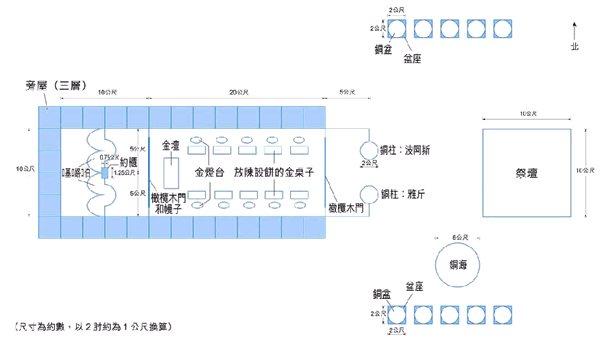
\includegraphics[width=6in]{BLiShiFigs/SD}
\caption{所羅門聖殿}
\label{fig:sub2}
\end{subfigure}\\[1ex]
\begin{subfigure}{\linewidth}
\centering
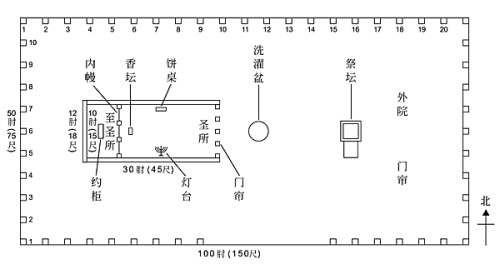
\includegraphics[width=6in]{BLiShiFigs/humu}
\caption{摩西會幕}
\label{fig:sub3}
\end{subfigure}
\label{fig:test}
\end{figure}
	 

%\subsubsection{運送聖器具及約櫃 5 }


\subsubsection{献殿 5}
\begin{table}[H]
\centering 
\begin{tabular}{|c|c|}\hline\hline
大衛分別為聖的金銀和器皿  &  放在神殿的府庫裡\\\hline
約櫃(裡有兩塊石版)從大衛城就是錫安運上來   &  至聖所,放在兩個基路伯的翅膀底下     \\\hline
會幕和會幕的一切聖器具都帶上來&     \\\hline
利未人亞薩、希幔、耶杜頓，和他們的眾子眾弟兄，敲鈸、鼓瑟、彈琴&站在壇的東邊  \\\hline
和華的榮光充滿&神的殿\\\hline
\end{tabular}
%\caption{運送聖器具及約櫃}
\end{table}
\subsubsubsection{殿工告竣，舁櫃入殿 5:1-10}
所羅門做完了耶和華殿的一切工，就把他父大衛分別為聖的金銀和器皿都帶來，放在神殿的府庫裡。
那時，所羅門將以色列的長老、各支派的首領並以色列的族長招聚到耶路撒冷，要把耶和華的約櫃從大衛城，就是錫安，運上來。 3 於是以色列眾人在七月節前都聚集到王那裡。 4 以色列眾長老來到，利未人便抬起約櫃。 5 祭司利未人將約櫃運上來，又將會幕和會幕的一切聖器具都帶上來。 6 所羅門王和聚集到他那裡的以色列全會眾，都在約櫃前獻牛羊為祭，多得不可勝數。 7 祭司將耶和華的約櫃抬進內殿，就是至聖所，放在兩個基路伯的翅膀底下。 8 基路伯張著翅膀在約櫃之上，遮掩約櫃和抬櫃的槓。 9 這槓甚長，槓頭在內殿前可以看見，在殿外卻不能看見，直到如今還在那裡。 10 約櫃裡唯有兩塊石版，就是以色列人出埃及後，耶和華與他們立約的時候，摩西在何烈山所放的，除此以外，並無別物。

\subsubsubsection{祭司利未人供職，耶和華的榮光充滿神殿 5:11-14}
當時在那裡所有的祭司都已自潔，並不分班供職。他們出聖所的時候，歌唱的利未人亞薩、希幔、耶杜頓和他們的眾子、眾弟兄都穿細麻布衣服，站在壇的東邊，敲鈸、鼓瑟、彈琴，同著他們有一百二十個祭司吹號。吹號的、歌唱的都一齊發聲，聲合為一，讚美、感謝耶和華。吹號、敲鈸，用各種樂器，揚聲讚美耶和華說：「耶和華本為善，他的慈愛永遠長存！」那時耶和華的殿有雲充滿，甚至祭司不能站立供職，因為耶和華的榮光充滿了神的殿。







\subsubsubsection{所羅門為民祝福 6:1-11}
\begin{table}[H]

\centering
\begin{tabular}{p{3cm}|p{14.cm}}\hline\hline
祝福&赞美神的拣选和成就了應許　\\\hline\hline
\multirow{2}{3.1cm}{那時所羅門說：「耶和華曾說他必住在幽暗之處。但我已經建造殿宇做你的居所，為你永遠的住處。」王轉臉為以色列會眾祝福，以色列會眾就都站立。}&所羅門說：「耶和華以色列的神是應當稱頌的！因他親口向我父大衛所應許的，也親手成就了。他說：『自從我領我民出埃及地以來，我未曾在以色列眾支派中選擇一城建造殿宇為我名的居所，也未曾揀選一人做我民以色列的君。但選擇耶路撒冷為我名的居所，又揀選大衛治理我民以色列。』」\\\cline{2-2}
&所羅門說：「我父大衛曾立意要為耶和華以色列神的名建殿，耶和華卻對我父大衛說：『你立意要為我的名建殿，這意思甚好，只是你不可建殿，唯你所生的兒子，必為我名建殿。』現在耶和華成就了他所應許的話，使我接續我父大衛坐以色列的國位，是照耶和華所說的，又為耶和華以色列神的名建造了殿。 11 我將約櫃安置在其中，櫃內有耶和華的約，就是他與以色列人所立的約。」\\\hline
\end{tabular}
\end{table}

\subsubsubsection{所羅門為民祈禱 6:12-242}
所羅門當著以色列會眾，站在耶和華的壇前，舉起手來。 13 所羅門曾造一個銅臺，長五肘，寬五肘，高三肘，放在院中，就站在臺上，當著以色列的會眾跪下，向天舉手， 14 說：「耶和華以色列的神啊，天上地下，沒有神可比你的。你向那盡心行在你面前的僕人守約施慈愛， 15 向你僕人我父大衛所應許的話現在應驗了。你親口應許，親手成就，正如今日一樣。 16 耶和華以色列的神啊，你所應許你僕人我父大衛的話說『你的子孫若謹慎自己的行為，遵守我的律法，像你在我面前所行的一樣，就不斷人坐以色列的國位』，現在求你應驗這話。 17 耶和華以色列的神啊，求你成就向你僕人大衛所應許的話！ 「神果真與世人同住在地上嗎？看哪，天和天上的天尚且不足你居住的，何況我所建的這殿呢！ 19 唯求耶和華我的神垂顧僕人的禱告、祈求，俯聽僕人在你面前的祈禱、呼籲。 20 願你晝夜看顧這殿，就是你應許立為你名的居所；求你垂聽僕人向此處禱告的話。 21 你僕人和你民以色列向此處祈禱的時候，求你從天上你的居所垂聽，垂聽而赦免。


%\subsubsubsection{所羅門禱告的内容 6:22-39}
\begin{table}[H]
\centering 
\begin{tabular}{p{4cm}|p{7cm}|p{6.25cm}}\hline\hline
各種境況 & 禱告蒙應允的條件 & 向神的祈求\\\hline\hline
人若得罪鄰舍，有人叫他起誓&    他來到這殿，在你的壇前起誓&求你從天上垂聽，判斷你的僕人，定惡人有罪，照他所行的報應在他頭上；定義人有理，照他的義賞賜他。 \\\hline
你的民以色列若得罪你，敗在仇敵面前&回心轉意承認你的名，在這殿裡向你祈求禱告&求你從天上垂聽，赦免你民以色列的罪，使他們歸回你賜給他們和他們列祖之地  \\\hline
你的民因得罪你，你懲罰他們，使天閉塞不下雨&他們若向此處禱告，承認你的名，離開他們的罪&求你在天上垂聽，赦免你僕人和你民以色列的罪，將當行的善道指教他們，且降雨在你的地，就是你賜給你民為業之地\\\hline
國中若有饑荒、瘟疫、旱風、霉爛、蝗蟲、螞蚱，或有仇敵犯境，圍困城邑，無論遭遇什麼災禍疾病&你的民以色列，或是眾人，或是一人，自覺災禍甚苦，向這殿舉手，無論祈求什麼，禱告什麼&求你從天上你的居所垂聽赦免。你是知道人心的，要照各人所行的待他們,使他們在你賜給我們列祖之地上一生一世敬畏你，遵行你的道\\\hline
論到不屬你民以色列的外邦人&為你的大名和大能的手，並伸出來的膀臂，從遠方而來，向這殿禱告  &求你從天上你的居所垂聽，照著外邦人所祈求的而行，使天下萬民都認識你的名，敬畏你，像你的民以色列一樣，又使他們知道我建造的這殿是稱為你名下的\\\hline
你的民若奉你的差遣，無論往何處去與仇敵爭戰& 向你所選擇的城與我為你名所建造的殿禱告 &求你從天上垂聽他們的禱告祈求，使他們得勝\\\hline
你的民若得罪你（世上沒有不犯罪的人），你向他們發怒，將他們交給仇敵擄到或遠或近之地 & 他們若在擄到之地想起罪來，回心轉意，懇求你說：『我們有罪了，我們悖逆了，我們作惡了』 他們若在擄到之地盡心盡性歸服你，又向自己的地，就是你賜給他們列祖之地和你所選擇的城，並我為你名所建造的殿禱告； &求你從天上你的居所垂聽你民的禱告祈求，為他們伸冤，赦免他們的過犯  \\\hline
\end{tabular}
%\caption{所羅門的禱告}
\end{table}

%\subsubsubsection{所羅門禱告的内容 6:22-39}
40 「我的神啊，現在求你睜眼看、側耳聽在此處所獻的禱告。 41 耶和華神啊，求你起來，和你有能力的約櫃同入安息之所。耶和華神啊，願你的祭司披上救恩，願你的聖民蒙福歡樂。 42 耶和華神啊，求你不要厭棄你的受膏者，要記念向你僕人大衛所施的慈愛。」

\subsubsection{耶和華榮光充滿殿宇 7:1-3}
\begin{table}[H]
\centering 
\begin{tabular}{p{3.75cm}|p{13.5cm}}\hline\hline
主角 &事件\\\hline\hline
耶和華  &  所羅門祈禱已畢，就有火從天上降下來，燒盡燔祭和別的祭。耶和華的榮光充滿了殿\\\hline
以色列眾人   &看見，就在鋪石地俯伏叩拜，稱謝耶和華說：耶和華本為善，他的慈愛永遠長存！    \\\hline
王和眾民& 在耶和華面前獻祭    \\\hline
祭司& 侍立，各供其職,在眾人面前吹號\\\hline
利未人&拿著耶和華的樂器,頌讚耶和華\\\hline
所羅門和以色列眾人&從哈馬口直到埃及小河，所有的以色列人都聚集成為大會，守節七日。第八日設立嚴肅會，行奉獻壇的禮七日，守節七日\\\hline
\end{tabular}
%\caption{獻殿禮}
\end{table}
所羅門祈禱已畢，就有火從天上降下來，燒盡燔祭和別的祭，耶和華的榮光充滿了殿。 2 因耶和華的榮光充滿了耶和華殿，所以祭司不能進殿。 3 那火降下，耶和華的榮光在殿上的時候，以色列眾人看見，就在鋪石地俯伏叩拜，稱謝耶和華說：「耶和華本為善，他的慈愛永遠長存！」

\subsubsection{所羅門與民獻祭 7:4-7}
王和眾民在耶和華面前獻祭。 5 所羅門王用牛二萬二千、羊十二萬獻祭。這樣，王和眾民為神的殿行奉獻之禮。 6 祭司侍立，各供其職。利未人也拿著耶和華的樂器，就是大衛王造出來藉利未人頌讚耶和華的：「他的慈愛永遠長存！」祭司在眾人面前吹號，以色列人都站立。 7 所羅門因他所造的銅壇容不下燔祭、素祭和脂油，便將耶和華殿前院子當中分別為聖，在那裡獻燔祭和平安祭牲的脂油。

\subsubsection{集民守節，眾民都心中喜樂 7:8-10}
那時所羅門和以色列眾人，就是從哈馬口直到埃及小河所有的以色列人，都聚集成為大會，守節七日。 9 第八日設立嚴肅會，行奉獻壇的禮七日，守節七日。 10 七月二十三日，王遣散眾民。他們因見耶和華向大衛和所羅門與他民以色列所施的恩惠，就都心中喜樂，各歸各家去了。

\subsection{神二次向所羅門顯現 7:11-22 }
\begin{table}[H]
\centering 
\begin{tabular}{p{2.6cm}|p{5.5cm}|p{9.25cm}}\hline\hline
神向所羅門顯現& 條件 &結果\\\hline\hline
\multirow{3}{2.65cm}{所羅門造成了耶和華殿和王宮，在耶和華殿和王宮凡他心中所要做的，都順順利利地做成了。夜間，耶和華向所羅門顯現，對他說：「我已聽了你的禱告，也選擇這地方作為祭祀我的殿宇。}
&我若使天閉塞不下雨，或使蝗蟲吃這地的出產，或使瘟疫流行在我民中，這稱為我名下的子民，若是自卑，禱告，尋求我的面，轉離他們的惡行，
&我必從天上垂聽，赦免他們的罪，醫治他們的地。我必睜眼看、側耳聽在此處所獻的禱告。現在我已選擇這殿，分別為聖，使我的名永在其中，我的眼、我的心也必常在那裡。\\\cline{2-3}　
&你若在我面前效法你父大衛所行的，遵行我一切所吩咐你的，謹守我的律例、典章，&我就必堅固你的國位，正如我與你父大衛所立的約說：『你的子孫必不斷人做以色列的王。』\\\cline{2-3}　
&倘若你們轉去，丟棄我指示你們的律例、誡命，去侍奉敬拜別神，&我就必將以色列人從我賜給他們的地上拔出根來，並且我為己名所分別為聖的殿也必捨棄不顧，使他在萬民中做笑談，被譏誚。這殿雖然甚高，將來經過的人必驚訝，說：『耶和華為何向這地和這殿如此行呢？』人必回答說：『是因此地的人離棄耶和華他們列祖的神，就是領他們出埃及地的神，去親近別神，敬拜侍奉他，所以耶和華使這一切災禍臨到他們。』\\\hline
\end{tabular}
%\caption{神二次向所羅門顯現}
\end{table}


\subsection{所羅門其他政績 8}
   \begin{figure}[H]  
	 \begin{center}
	 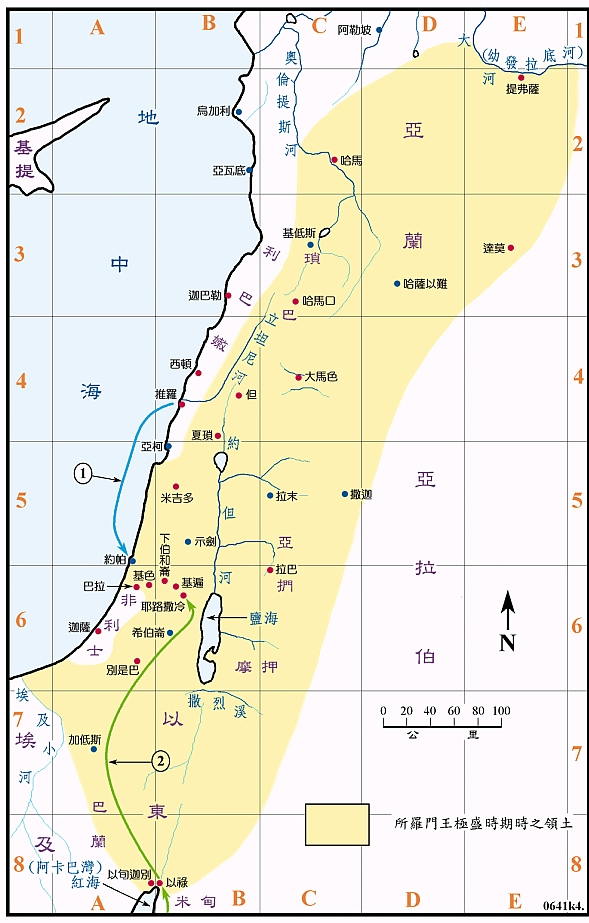
\includegraphics[width=3in]{BLiShiFigs/suoluomen}
	 \label{fig:1} 
	 \end{center}
	 \end{figure}

\subsubsection{所羅門建邑 8:1-6}
\begin{table}[H]
\centering 
\begin{tabular}{ p{14cm} }\hline\hline
建造耶和華殿和王宮\\\hline　
重新修築希蘭送給他的那些城邑，使以色列人住在那裡  \\\hline
往哈馬瑣巴去，攻取了那地方 \\\hline
建造曠野裡的達莫，又建造哈馬所有的積貨城\\\hline
建造上伯和崙、下伯和崙作為保障\\\hline
 建造巴拉和所有的積貨城，並屯車輛馬兵的城\\\hline
 建造與耶路撒冷、利巴嫩以及自己治理的全國中所願意建造的\\\hline
 不屬以色列人的挑取他們的後裔作服苦的奴僕; 以色列人作他的戰士、軍長的統領、車兵長、馬兵長\\\hline
 \end{tabular}
\end{table}
所羅門建造耶和華殿和王宮，二十年才完畢了。 2 以後所羅門重新修築希蘭送給他的那些城邑，使以色列人住在那裡。

3 所羅門往哈馬瑣巴去，攻取了那地方。 4 所羅門建造曠野裡的達莫，又建造哈馬所有的積貨城。 5 又建造上伯和崙、下伯和崙作為保障，都有牆、有門、有閂。 6 又建造巴拉和所有的積貨城，並屯車輛馬兵的城，與耶路撒冷、黎巴嫩，以及自己治理的全國中所願意建造的。

\subsubsection{徵異族人服役，帶法老女兒出大衛城 8:7-11}
至於國中所剩下不屬以色列人的赫人、亞摩利人、比利洗人、希未人、耶布斯人， 8 就是以色列人未曾滅絕的，所羅門挑取他們的後裔做服苦的奴僕，直到今日。 9 唯有以色列人，所羅門不使他們當奴僕做工，乃是做他的戰士、軍長的統領、車兵長、馬兵長。 10 所羅門王有二百五十督工的，監管工人。

11 所羅門將法老的女兒帶出大衛城，上到為他建造的宮裡，因所羅門說：「耶和華約櫃所到之處都為聖地，所以我的妻不可住在以色列王大衛的宮裡。」

\subsubsection{獻燔祭,定祭司之班利未人之職 8:12-16}
\begin{table}[H]
\centering 
\begin{tabular}{p{5.25cm}|p{8.5cm}|p{3cm}}\hline\hline
守節，獻祭&派定祭司的班次&建殿完畢\\\hline\hline
所羅門在耶和華的壇上，就是在廊子前他所築的壇上，與耶和華獻燔祭，又遵著摩西的吩咐，在安息日、月朔並一年三節，就是除酵節、七七節、住棚節，獻每日所當獻的祭。
&所羅門照著他父大衛所定的例，派定祭司的班次，使他們各供己事，又使利未人各盡其職，讚美耶和華，在祭司面前做每日所當做的，又派守門的按著班次看守各門，因為神人大衛是這樣吩咐的。王所吩咐眾祭司和利未人的，無論是管府庫或辦別的事，他們都不違背。
&所羅門建造耶和華的殿，從立根基直到成功的日子，工料俱備。這樣，耶和華的殿全然完畢。\\\hline
\end{tabular}
\end{table}


\subsubsection{航海之船舶 8:17-18}

那時，所羅門往以東地靠海的以旬迦別和以祿去。 18 希蘭差遣他的臣僕，將船隻和熟悉泛海的僕人送到所羅門那裡。他們同著所羅門的僕人到了俄斐，得了四百五十他連得金子，運到所羅門王那裡。

	 
\subsection{示巴女王拜見所羅門 9:1-12 }
\begin{table}[H]
\centering 
\begin{tabular}{p{3.25cm}|p{2.65cm}|p{5.35cm}||p{5.25cm}}\hline\hline
示巴女王所聽&示巴女王所見&示巴女王所說&示巴女王所送\\\hline\hline
示巴女王聽見所羅門的名聲，就來到耶路撒冷，要用難解的話試問所羅門。跟隨她的人甚多，又有駱駝馱著香料、寶石和許多金子。她來見了所羅門，就把心裡所有的對所羅門都說出來。所羅門將她所問的都答上了，沒有一句不明白不能答的。
&示巴女王見所羅門的智慧，和他所建造的宮室，席上的珍饈美味，群臣分列而坐，僕人兩旁侍立，以及他們的衣服裝飾，酒政和酒政的衣服裝飾，又見他上耶和華殿的臺階，就詫異得神不守舍，
&對王說：「我在本國裡所聽見論到你的事和你的智慧實在是真的！我先不信那些話，及至我來，親眼見了，才知道你的大智慧，人所告訴我的還不到一半。你的實跡越過我所聽見的名聲。你的群臣、你的僕人常侍立在你面前聽你智慧的話是有福的！耶和華你的神是應當稱頌的！他喜悅你，使你坐他的國位，為耶和華你的神做王。因為你的神愛以色列人，要永遠堅立他們，所以立你做他們的王，使你秉公行義。」
&於是示巴女王將一百二十他連得金子和寶石，與極多的香料送給所羅門王。她送給王的香料，以後再沒有這樣的。希蘭的僕人和所羅門的僕人從俄斐運了金子來，也運了檀香木（烏木）和寶石來。王用檀香木為耶和華殿和王宮做臺，又為歌唱的人做琴瑟；猶大地從來沒有見過這樣的。所羅門王按示巴女王所帶來的還她禮物，另外照她一切所要所求的，都送給她。於是女王和她臣僕轉回本國去了。\\\hline
\end{tabular}
\end{table}



\subsection{所羅門的尊榮 9:13-21}
\begin{table}[H]
\centering 
\begin{tabular}{p{6.25cm}|p{5.25cm}|p{4.75cm}}\hline\hline
所羅門的金子&大寶座&飲器和其他所得\\\hline\hline
所羅門每年所得的金子共有六百六十六他連得，另外還有商人所進的金子，並且阿拉伯諸王與屬國的省長都帶金銀給所羅門。所羅門王用錘出來的金子打成擋牌二百面，每面用金子六百舍客勒，又用錘出來的金子打成盾牌三百面，每面用金子三百舍客勒，都放在黎巴嫩林宮裡。
&王用象牙製造一個大寶座，用精金包裹。寶座有六層臺階，又有金腳凳，與寶座相連。寶座兩旁有扶手，靠近扶手有兩個獅子站立。六層臺階上有十二個獅子站立，每層有兩個，左邊一個，右邊一個。在列國中沒有這樣做的。
&所羅門王一切的飲器都是金的，黎巴嫩林宮裡的一切器皿都是精金的，所羅門年間銀子算不了什麼。因為王的船隻與希蘭的僕人一同往他施去，他施船隻三年一次裝載金銀、象牙、猿猴、孔雀回來。\\\hline
\end{tabular}
%\caption{所羅門的尊榮}
\end{table}
 

\subsection{列王咸欲聽其哲言 9:22-28}
\begin{table}[H]
\centering 
\begin{tabular}{p{6.75cm}|p{3.5cm}|p{2.5cm}|p{3.75cm}}\hline\hline
列王帶的貢物&武力&领土&其他各种财物\\\hline\hline
所羅門王的財寶與智慧勝過天下的列王。普天下的王都求見所羅門，要聽神賜給他智慧的話。他們各帶貢物，就是金器、銀器、衣服、軍械、香料、騾馬，每年有一定之例。
&所羅門有套車的馬四千棚，有馬兵一萬二千，安置在屯車的城邑和耶路撒冷，就是王那裡。 
&所羅門統管諸王，從大河到非利士地，直到埃及的邊界。
& 王在耶路撒冷使銀子多如石頭，香柏木多如高原的桑樹。有人從埃及和各國為所羅門趕馬群來。\\\hline
\end{tabular}
%\caption{所羅門的尊榮}
\end{table}


\subsection{所羅門卒其子羅波安繼位 9:29-31 }
所羅門其餘的事，自始至終，不都寫在先知拿單的書上和示羅人亞希雅的預言書上，並先見易多論尼八兒子耶羅波安的默示書上嗎？ 30 所羅門在耶路撒冷做以色列眾人的王共四十年。 31 所羅門與他列祖同睡，葬在他父大衛城裡。他兒子羅波安接續他做王。


%\section{所羅門（1-9)}
\section{羅波安 10-12 }
%\subsection{羅波安到示劍被立作王}
%\subsection{羅波安用嚴厲的話回覆以色列眾民}
\subsection{以色列人背叛大衛家 10:1-19}
羅波安往示劍去，因為以色列人都到了示劍，要立他做王。 2 尼八的兒子耶羅波安先前躲避所羅門王，逃往埃及，住在那裡，他聽見這事，就從埃及回來。 3 以色列人打發人去請他，他就和以色列眾人來見羅波安，對他說： 4 「你父親使我們負重軛做苦工，現在求你使我們做的苦工、負的重軛輕鬆些，我們就侍奉你。」 5 羅波安對他們說：「第三日再來見我吧。」民就去了。

6 羅波安之父所羅門在世的日子，有侍立在他面前的老年人，羅波安王和他們商議，說：「你們給我出個什麼主意，我好回覆這民。」 7 老年人對他說：「王若恩待這民，使他們喜悅，用好話回覆他們，他們就永遠做王的僕人。」 8 王卻不用老年人給他出的主意，就和那些與他一同長大，在他面前侍立的少年人商議， 9 說：「這民對我說：『你父親使我們負重軛，求你使我們輕鬆些。』你們給我出個什麼主意，我好回覆他們。」 10 那同他長大的少年人說：「這民對王說：『你父親使我們負重軛，求你使我們輕鬆些。』王要對他們如此說：『我的小拇指比我父親的腰還粗！ 11 我父親使你們負重軛，我必使你們負更重的軛；我父親用鞭子責打你們，我要用蠍子鞭責打你們。』」

耶羅波安和眾百姓遵著羅波安王所說「你們第三日再來見我」的那話，第三日他們果然來了。 13 羅波安王用嚴厲的話回覆他們，不用老年人所出的主意， 14 照著少年人所出的主意對他們說：「我父親使你們負重軛，我必使你們負更重的軛；我父親用鞭子責打你們，我要用蠍子鞭責打你們。」 15 王不肯依從百姓，這事乃出於神，為要應驗耶和華藉示羅人亞希雅對尼八兒子耶羅波安所說的話。

\subsection{以色列人叛 10:16-19}
以色列眾民見王不依從他們，就對王說：「我們與大衛有什麼份兒呢？與耶西的兒子並沒有關涉！以色列人哪，各回各家去吧！大衛家啊，自己顧自己吧！」於是，以色列眾人都回自己家裡去了。 17 唯獨住在猶大城邑的以色列人，羅波安仍做他們的王。 18 羅波安王差遣掌管服苦之人的哈多蘭往以色列人那裡去，以色列人就用石頭打死他。羅波安王急忙上車，逃回耶路撒冷去了。 19 這樣，以色列人背叛大衛家，直到今日。


\subsection{神人示瑪雅禁羅波安與以色列人爭戰 11:1-4}
羅波安來到耶路撒冷，招聚猶大家和便雅憫家，共十八萬人，都是挑選的戰士，要與以色列人爭戰，好將國奪回再歸自己。 2 但耶和華的話臨到神人示瑪雅說： 3 「你去告訴所羅門的兒子猶大王羅波安和住猶大、便雅憫的以色列眾人說： 4 『耶和華如此說：你們不可上去與你們的弟兄爭戰。各歸各家去吧，因為這事出於我。』」眾人就聽從耶和華的話歸回，不去與耶羅波安爭戰。


\subsection{羅波安在猶大地修築城邑 11:5-12}
羅波安住在耶路撒冷，在猶大地修築城邑， 6 為保障修築伯利恆、以坦、提哥亞、 7 伯夙、梭哥、亞杜蘭、 8 迦特、瑪利沙、西弗、 9 亞多萊音、拉吉、亞西加、 10 瑣拉、亞雅崙、希伯崙，這都是猶大和便雅憫的堅固城。 11 羅波安又堅固各處的保障，在其中安置軍長，又預備下糧食、油、酒。 12 他在各城裡預備盾牌和槍，且使城極其堅固。猶大和便雅憫都歸了他。


%\subsection{神使羅波安強盛三年}
\subsection{祭司及利未人歸附羅波安 11:13-17}
以色列全地的祭司和利未人都從四方來歸羅波安。 14 利未人撇下他們的郊野和產業，來到猶大與耶路撒冷，是因耶羅波安和他的兒子拒絕他們，不許他們供祭司職分侍奉耶和華。 15 耶羅波安為丘壇，為鬼魔（公山羊），為自己所鑄造的牛犢，設立祭司。 16 以色列各支派中，凡立定心意尋求耶和華以色列神的，都隨從利未人來到耶路撒冷，祭祀耶和華他們列祖的神。 17 這樣，就堅固猶大國，使所羅門的兒子羅波安強盛三年，因為他們三年遵行大衛和所羅門的道。


\subsection{羅波安的家室 11:18-23}
\begin{forest}
  for tree={
    child anchor=west,
    parent anchor=east,
    grow=east,
    draw,
    anchor=west,
    edge path={
      \noexpand\path[\forestoption{edge}]
        (.child anchor) -| +(-5pt,0) -- +(-5pt,0) |-
        (!u.parent anchor)\forestoption{edge label};
    },
  }
  [羅波安[大衛兒子耶利摩的女兒瑪哈拉(妻)]
  			[耶西兒子以利押的女兒亞比孩(妻)[耶烏施][示瑪利雅][撒罕]]
			[押沙龍的女兒她瑪和基比亞人烏列女兒瑪迦(妻)[亞太][亞比雅(太子)][細撒][示羅密]]
  ]
\end{forest}
羅波安娶大衛兒子耶利摩的女兒瑪哈拉為妻，又娶耶西兒子以利押的女兒亞比孩為妻。 19 從她生了幾個兒子，就是耶烏施、示瑪利雅、撒罕。 20 後來又娶押沙龍的女兒瑪迦（13:2作「烏列的女兒米該雅」），從她生了亞比雅、亞太、細撒、示羅密。 21 羅波安娶十八個妻，立六十個妾，生二十八個兒子、六十個女兒，他卻愛押沙龍的女兒瑪迦比愛別的妻妾更甚。 22 羅波安立瑪迦的兒子亞比雅做太子，在他弟兄中為首，因為想要立他接續做王。 23 羅波安辦事精明，使他眾子分散在猶大和便雅憫全地各堅固城裡，又賜他們許多糧食，為他們多尋妻子。

\subsection{羅波安王第五年，埃及王示撒攻打耶路撒冷 12:1-12}
羅波安的國堅立，他強盛的時候就離棄耶和華的律法，以色列人也都隨從他。羅波安王第五年，埃及王示撒上來攻打耶路撒冷，因為王和民得罪了耶和華。 3 示撒帶戰車一千二百輛、馬兵六萬，並且跟從他出埃及的路比人、蘇基人和古實人多得不可勝數。 4 他攻取了猶大的堅固城，就來到耶路撒冷。 5 那時猶大的首領因為示撒就聚集在耶路撒冷，有先知示瑪雅去見羅波安和眾首領，對他們說：「耶和華如此說：你們離棄了我，所以我使你們落在示撒手裡。」 6 於是王和以色列的眾首領都自卑，說：「耶和華是公義的。」 7 耶和華見他們自卑，耶和華的話就臨到示瑪雅說：「他們既自卑，我必不滅絕他們，必使他們略得拯救。我不藉著示撒的手將我的怒氣倒在耶路撒冷。 8 然而他們必做示撒的僕人，好叫他們知道服侍我與服侍外邦人有何分別。」
於是埃及王示撒上來攻取耶路撒冷，奪了耶和華殿和王宮裡的寶物，盡都帶走，又奪去所羅門製造的金盾牌。 10 羅波安王製造銅盾牌代替那金盾牌，交給守王宮門的護衛長看守。 11 王每逢進耶和華的殿，護衛兵就拿這盾牌，隨後仍將盾牌送回，放在護衛房。 12 王自卑的時候，耶和華的怒氣就轉消了，不將他滅盡；並且在猶大中間也有善益的事。

\subsection{羅波安去世 12:13-16}
羅波安王自強，在耶路撒冷做王。他登基的時候年四十一歲，在耶路撒冷，就是耶和華從以色列眾支派中所選擇立他名的城，做王十七年。羅波安的母親名叫拿瑪，是亞捫人。 14 羅波安行惡，因他不立定心意尋求耶和華。羅波安所行的事，自始至終，不都寫在先知示瑪雅和先見易多的史記上嗎？羅波安與耶羅波安時常爭戰。 16 羅波安與他列祖同睡，葬在大衛城裡。他兒子亞比雅接續他做王。

\section{亞比雅（亞比央） 13 }
\subsection{亞比雅做猶大王三年 13:1-2}

耶羅波安王十八年，亞比雅登基做猶大王， 2 在耶路撒冷做王三年。他母親名叫米該亞 （瑪迦），是基比亞人烏列的女兒。亞比雅常與耶羅波安爭戰。

\subsection{亞比雅與耶羅波安爭戰 13:3-20}
\begin{figure}
\centering
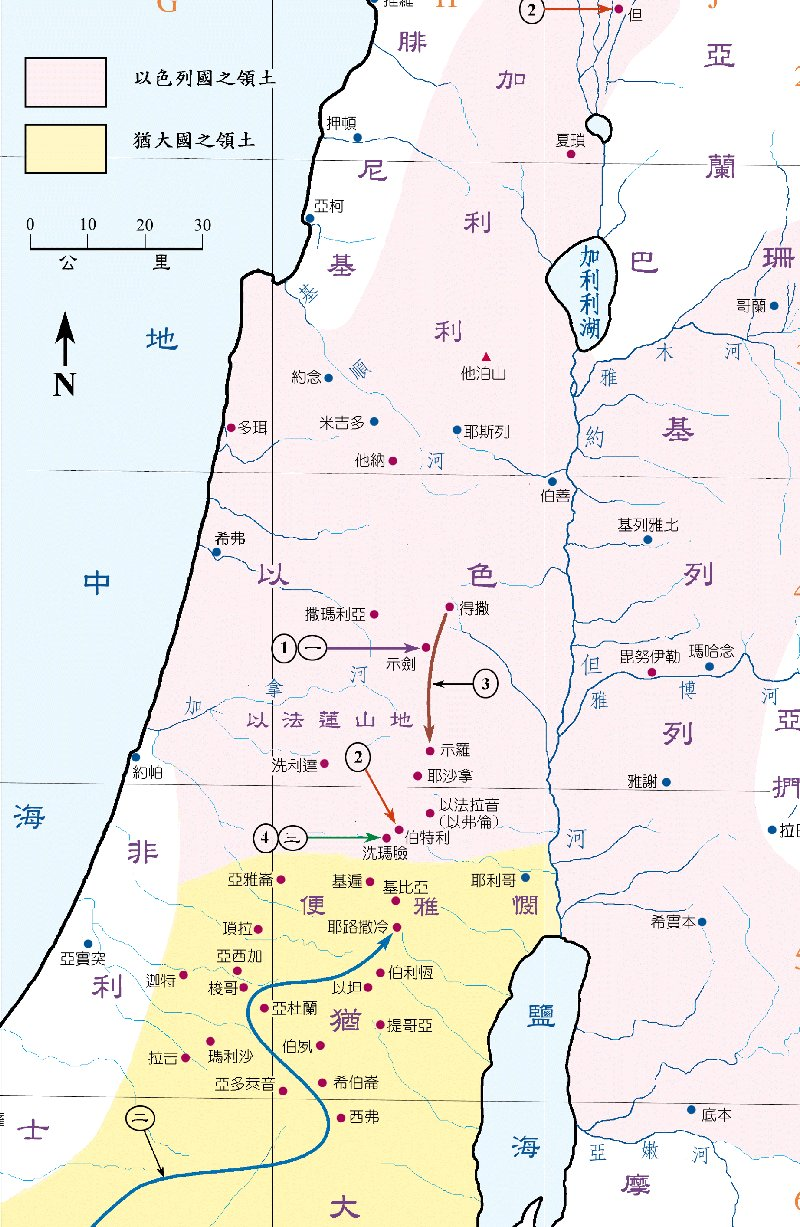
\includegraphics[width=5.8in]{BLiShiFigs/yabiyang}
\caption{亞比雅與耶羅波安爭戰}
\label{fig:sub1}
\end{figure}
\subsubsection{亞比雅四十萬與耶羅波安八十萬擺陣 13:3-20}
\begin{table}[H]
\centering 
\begin{tabular}{p{1.75cm}|p{15.5cm}}\hline\hline
双方擺陣&亞比雅的讲论\\\hline\hline
\multirow{3}{1.9cm}{有一次亞比雅率領挑選的兵四十萬擺陣，都是勇敢的戰士，耶羅波安也挑選大能的勇士八十萬，對亞比雅擺陣。}
&亞比雅站在以法蓮山地中的洗瑪臉山上說：「耶羅波安和以色列眾人哪，要聽我說！耶和華以色列的神曾立鹽（不廢壞）約，將以色列國永遠賜給大衛和他的子孫，你們不知道嗎？無奈大衛兒子所羅門的臣僕，尼八兒子耶羅波安起來背叛他的主人。有些無賴的匪徒聚集跟從他，逞強攻擊所羅門的兒子羅波安，那時羅波安還幼弱，不能抵擋他們。\\\cline{2-2}
&現在你們有意抗拒大衛子孫手下所治耶和華的國，你們的人也甚多，你們那裡又有耶羅波安為你們所造當做神的金牛犢。你們不是驅逐耶和華的祭司亞倫的後裔和利未人嗎？不是照著外邦人的惡俗為自己立祭司嗎？無論何人牽一隻公牛犢、七隻公綿羊將自己分別出來，就可做虛無之神的祭司。\\\cline{2-2}
&至於我們，耶和華是我們的神，我們並沒有離棄他。我們有侍奉耶和華的祭司，都是亞倫的後裔，並有利未人各盡其職，每日早晚向耶和華獻燔祭燒美香，又在精金的桌子上擺陳設餅，又有金燈臺和燈盞，每晚點起。因為我們遵守耶和華我們神的命，唯有你們離棄了他。 率領我們的是神，我們這裡也有神的祭司拿號向你們吹出大聲。以色列人哪不要與耶和華你們列祖的神爭戰，因你們必不能亨通！」\\\hline
\end{tabular}
%\caption{所羅門的尊榮}
\end{table}
 

\subsection{猶大人呼求耶和華，以色列人敗遁 13:13-20}
\begin{table}[H]
\centering 
\begin{tabular}{p{4.65cm}|p{7.15cm}|p{5.5cm}}\hline\hline
双方擺陣&猶大人呼求耶和華就得勝&\\\hline\hline
耶羅波安卻在猶大人的後頭設伏兵，這樣以色列人在猶大人的前頭，伏兵在猶大人的後頭。猶大人回頭觀看，見前後都有敵兵，就呼求耶和華，祭司也吹號。於是猶大人呐喊。
&猶大人呐喊的時候神就使耶羅波安和以色列眾人敗在亞比雅與猶大人面前。以色列人在猶大人面前逃跑，神將他們交在猶大人手裡。亞比雅和他的軍兵大大殺戮以色列人，以色列人仆倒死亡的精兵有五十萬。那時以色列人被制伏了，猶大人得勝是因倚靠耶和華他們列祖的神。
&亞比雅追趕耶羅波安攻取了他的幾座城,就是伯特利和屬伯特利的鎮市,耶沙拿和屬耶沙拿的鎮市,以法拉音（以弗倫）和屬以法拉音的鎮市。亞比雅在世的時候耶羅波安不能再強盛。耶和華攻擊他,他就死了。 
\\\hline
\end{tabular}
%\caption{所羅門的尊榮}
\end{table}



\subsection{亞比雅的家室 13:21-22}
亞比雅卻漸漸強盛，娶妻妾十四個，生了二十二個兒子、十六個女兒。 22 亞比雅其餘的事和他的言行都寫在先知易多的傳上。




\section{亞撒 14-16 }
\subsection{亞撒繼位和他的政績 14:1-8}
\begin{table}[H]
\centering 
\begin{tabular}{p{2.35cm}|p{5.25cm}|p{6.55cm}|p{2.85cm}}\hline\hline
亞撒做王&尋求耶和華耶和華&建造城樓&軍兵勇士\\\hline\hline
亞比雅與他列祖同睡，葬在大衛城裡。他兒子亞撒接續他做王。亞撒年間，國中太平十年。
&亞撒行耶和華他神眼中看為善為正的事，除掉外邦神的壇和丘壇，打碎柱像，砍下木偶，吩咐猶大人尋求耶和華他們列祖的神，遵行他的律法、誡命，又在猶大各城邑除掉丘壇和日像，那時國享太平。
&又在猶大建造了幾座堅固城。國中太平數年，沒有戰爭，因為耶和華賜他平安。他對猶大人說：「我們要建造這些城邑，四圍築牆，蓋樓、安門做閂。地還屬我們，是因尋求耶和華我們的神；我們既尋求他，他就賜我們四境平安。」於是建造城邑，諸事亨通。&亞撒的軍兵，出自猶大拿盾牌拿槍的三十萬人，出自便雅憫拿盾牌拉弓的二十八萬人，這都是大能的勇士。\\\hline
\end{tabular}
\end{table}



 

\subsection{亞撒戰勝古實王謝拉一百萬軍兵 14:9-14}
\begin{table}[H]
\centering 
\begin{tabular}{p{3.5cm}|p{5.cm}|p{8.5cm}}\hline\hline
古實王謝拉攻擊猶大&亞撒呼求耶和華他的神&古實人敗\\\hline\hline
有古實王謝拉率領軍兵一百萬、戰車三百輛，出來攻擊猶大人，到了瑪利沙。於是亞撒出去與他迎敵，就在瑪利沙的洗法谷彼此擺陣。
&亞撒呼求耶和華他的神，說：「耶和華啊，唯有你能幫助軟弱的勝過強盛的。耶和華我們的神啊，求你幫助我們，因為我們仰賴你，奉你的名來攻擊這大軍。耶和華啊，你是我們的神，不要容人勝過你。」
&於是耶和華使古實人敗在亞撒和猶大人面前，古實人就逃跑了。亞撒和跟隨他的軍兵追趕他們，直到基拉耳。古實人被殺的甚多，不能再強盛，因為敗在耶和華與他軍兵面前。猶大人就奪了許多財物。又打破基拉耳四圍的城邑，耶和華使其中的人都甚恐懼。猶大人又將所有的城擄掠一空，因其中的財物甚多。又毀壞了群畜的圈，奪取許多的羊和駱駝，就回耶路撒冷去了。\\\hline
\end{tabular}
%\caption{所羅門的尊榮}
\end{table}


\subsection{先知亞撒利雅勸誡亞撒 15:1-7}
\begin{table}[H]
\centering 
\begin{tabular}{p{6.5cm}|p{8.5cm}|p{2.cm}}\hline\hline
順從耶和華&神用各樣災難擾亂列國&要剛強，得賞賜\\\hline\hline
神的靈感動俄德的兒子亞撒利雅，他出來迎接亞撒，對他說：「亞撒和猶大、便雅憫眾人哪，要聽我說！你們若順從耶和華，耶和華必與你們同在。你們若尋求他，就必尋見；你們若離棄他，他必離棄你們。
&以色列人不信真神，沒有訓誨的祭司，也沒有律法，已經好久了，但他們在急難的時候歸向耶和華以色列的神，尋求他，他就被他們尋見。那時，出入的人不得平安，列國的居民都遭大亂，這國攻擊那國，這城攻擊那城，互相破壞，因為神用各樣災難擾亂他們。
&現在你們要剛強，不要手軟，因你們所行的必得賞賜。」\\\hline
\end{tabular}
%\caption{所羅門的尊榮}
\end{table}


\subsection{亞撒納先知勸勉,除可憎之物，聚眾向神立約 15:8-15}
\begin{table}[H]
\centering 
\begin{tabular}{p{4.cm}|p{5.5cm}|p{5.5cm}|p{1.25cm}}\hline\hline
納先知勸勉&聚眾&立約&耶和華\\\hline\hline
亞撒聽見這話和俄德兒子先知亞撒利雅的預言，就壯起膽來，在猶大、便雅憫全地並以法蓮山地所奪的各城，將可憎之物盡都除掉，又在耶和華殿的廊前重新修築耶和華的壇。
&又招聚猶大、便雅憫的眾人，並他們中間寄居的以法蓮人、瑪拿西人、西緬人：有許多以色列人歸降亞撒，因見耶和華他的神與他同在。亞撒十五年三月，他們都聚集在耶路撒冷。當日，他們從所取的擄物中將牛七百隻、羊七千隻獻給耶和華。
&他們就立約，要盡心、盡性地尋求耶和華他們列祖的神，凡不尋求耶和華以色列神的，無論大小、男女，必被治死。他們就大聲歡呼，吹號吹角，向耶和華起誓。猶大眾人為所起的誓歡喜。因他們是盡心起誓，盡意尋求耶和華，
&耶和華就被他們尋見，且賜他們四境平安。\\\hline
\end{tabular}
%\caption{所羅門的尊榮}
\end{table}


\subsection{亞撒貶祖母瑪迦之后位 15:16-19}
亞撒王貶了他祖母瑪迦太后的位，因她造了可憎的偶像亞舍拉。亞撒砍下她的偶像，搗得粉碎，燒在汲淪溪邊。 17 只是丘壇還沒有從以色列中廢去，然而亞撒的心一生誠實。 18 亞撒將他父所分別為聖與自己所分別為聖的金銀和器皿，都奉到神的殿裡。 19 從這時直到亞撒三十五年，都沒有爭戰的事。

\subsection{以色列王巴沙攻猶大,亞撒求助於亞蘭王 16:1-6}
\begin{table}[H]
\centering 
\begin{tabular}{p{4.cm}|p{8.25cm}|p{4.75cm}}\hline\hline
双方擺陣&猶大人呼求耶和華就得勝&\\\hline\hline
亞撒三十六年，以色列王巴沙上來攻擊猶大，修築拉瑪，不許人從猶大王亞撒那裡出入。
&於是亞撒從耶和華殿和王宮的府庫裡拿出金銀來，送於住大馬士革的亞蘭王便哈達，說： 「你父曾與我父立約，我與你也要立約。現在我將金銀送給你，求你廢掉你與以色列王巴沙所立的約，使他離開我。」
&便哈達聽從亞撒王的話，派軍長去攻擊以色列的城邑。他們就攻破以雲、但、亞伯瑪音和拿弗他利一切的積貨城。
\\\hline
巴沙聽見，就停工不修築拉瑪了。&於是亞撒王率領猶大眾人，將巴沙修築拉瑪所用的石頭、木頭都運去，用以修築迦巴和米斯巴。&\\\hline
\end{tabular}
%\caption{所羅門的尊榮}
\end{table}


\subsection{哈拿尼責猶大王亞撒 16:7-10}
\begin{table}[H]
\centering 
\begin{tabular}{p{13.5cm}|p{4.cm}}\hline\hline
哈拿尼責亞撒&亞撒惱恨先見\\\hline\hline
那時，先見哈拿尼來見猶大王亞撒，對他說：「因你仰賴亞蘭王，沒有仰賴耶和華你的神，所以亞蘭王的軍兵脫離了你的手。古實人、路比人的軍隊不是甚大嗎？戰車馬兵不是極多嗎？只因你仰賴耶和華，他便將他們交在你手裡。耶和華的眼目遍察全地，要顯大能幫助向他心存誠實的人。你這事行得愚昧，此後你必有爭戰的事。」
&亞撒因此惱恨先見，將他囚在監裡。那時，亞撒也虐待一些人民。\\\hline
\end{tabular}
%\caption{所羅門的尊榮}
\end{table}


\subsection{亞撒患腳病而死 16:11-14}
亞撒所行的事，自始至終，都寫在《猶大和以色列諸王記》上。 12 亞撒做王三十九年，他腳上有病，而且甚重。病的時候沒有求耶和華，只求醫生。 13 他做王四十一年而死，與他列祖同睡， 14 葬在大衛城自己所鑿的墳墓裡，放在床上，其床堆滿各樣馨香的香料，就是按做香的做法調和的香料，又為他燒了許多的物件。

\section{約沙法 17-20 }
\subsection{約沙法的功績 17}
\subsubsection{約沙法做猶大王 17:1-6}
亞撒的兒子約沙法接續他做王，奮勇自強，防備以色列人， 2 安置軍兵在猶大一切堅固城裡，又安置防兵在猶大地和他父亞撒所得以法蓮的城邑中。 3 耶和華與約沙法同在，因為他行他祖大衛初行的道，不尋求巴力， 4 只尋求他父親的神，遵行他的誡命，不效法以色列人的行為。 5 所以耶和華堅定他的國，猶大眾人給他進貢，約沙法大有尊榮、資財。 6 他高興遵行耶和華的道，並且從猶大除掉一切丘壇和木偶。

\subsubsection{做王第三年差人走遍猶大传讲律法 17:7-9}
\begin{wraptable}{r}{8cm}
\vspace{-10mm}
\centering
\begin{tabular}{p{1.25cm}|p{5.75cm}}\hline\hline
 職位& 名字\\\hline\hline
 臣子&便亥伊勒、俄巴底、撒迦利雅、拿坦業、米該亞 \\\hline
利未人&示瑪雅、尼探雅、西巴第雅、亞撒黑、示米拉末、約拿單、亞多尼雅、多比雅、駝巴多尼雅\\\hline
 祭司&以利沙瑪、約蘭\\\hline
\end{tabular} 
%\caption{受約沙法差遣教訓百姓的人員}
\end{wraptable}
他做王第三年，就差遣臣子便亥伊勒、俄巴底、撒迦利雅、拿坦業、米該亞往猶大各城去教訓百姓。 8 同著他們有利未人示瑪雅、尼探雅、西巴第雅、亞撒黑、示米拉末、約拿單、亞多尼雅、多比雅、駝巴多尼雅，又有祭司以利沙瑪、約蘭同著他們。 9 他們帶著耶和華的律法書，走遍猶大各城教訓百姓。

\subsubsection{列國畏其強盛臣服納貢 17:10-19}
耶和華使猶大四圍的列國都甚恐懼，不敢與約沙法爭戰。 11 有些非利士人與約沙法送禮物納貢銀，阿拉伯人也送他公綿羊七千七百隻、公山羊七千七百隻。 12 約沙法日漸強大，在猶大建造營寨和積貨城。 13 他在猶大城邑中有許多工程，又在耶路撒冷有戰士，就是大能的勇士。 14 他們的數目，按著宗族記在下面：猶大族的，千夫長押拿為首，率領大能的勇士三十萬； 15 其次是千夫長約哈難，率領大能的勇士二十八萬； 16 其次是細基利的兒子亞瑪斯雅，他為耶和華犧牲自己，率領大能的勇士二十萬。 17 便雅憫族，是大能的勇士以利雅大，率領拿弓箭和盾牌的二十萬； 18 其次是約薩拔，率領預備打仗的十八萬。 19 這都是伺候王的，還有王在猶大全地堅固城所安置的，不在其內。

\subsection{約沙法與亞哈 18:1-34}
\subsubsection{約沙法與亞哈結親 18:1-3}
約沙法大有尊榮、資財，就與亞哈結親。 2 過了幾年，他下到撒馬利亞去見亞哈。亞哈為他和跟從他的人宰了許多牛羊，勸他與自己同去攻取基列的拉末。 3 以色列王亞哈問猶大王約沙法說：「你肯同我去攻取基列的拉末嗎？」他回答說：「你我不分彼此，我的民與你的民一樣，必與你同去爭戰。」

\subsubsection{約沙法與亞哈求先知諮諏耶和華 18:4-11}
約沙法對以色列王說：「請你先求問耶和華。」 5 於是以色列王招聚先知四百人，問他們說：「我們上去攻取基列的拉末可以不可以？」他們說：「可以上去，因為神必將那城交在王的手裡。」 6 約沙法說：「這裡不是還有耶和華的先知我們可以求問他嗎？」 7 以色列王對約沙法說：「還有一個人，是音拉的兒子米該雅，我們可以託他求問耶和華。只是我恨他，因為他指著我所說的預言不說吉語，常說凶言。」約沙法說：「王不必這樣說。」 8 以色列王就召了一個太監來，說：「你快去將音拉的兒子米該雅召來。」 9 以色列王和猶大王約沙法在撒馬利亞城門前的空場上，各穿朝服，坐在位上，所有的先知都在他們面前說預言。 10 基拿拿的兒子西底家造了兩個鐵角，說：「耶和華如此說：你要用這角牴觸亞蘭人，直到將他們滅盡。」 11 所有的先知也都這樣預言說：「可以上基列的拉末去，必然得勝，因為耶和華必將那城交在王的手中。」

\subsubsection{米該雅之警戒 18:12-22}
那去召米該雅的使者對米該雅說：「眾先知一口同音地都向王說吉言，你不如與他們說一樣的話，也說吉言。」 13 米該雅說：「我指著永生的耶和華起誓：我的神說什麼，我就說什麼。」 14 米該雅到王面前，王問他說：「米該雅啊，我們上去攻取基列的拉末可以不可以？」他說：「可以上去，必然得勝，敵人必交在你們手裡。」 15 王對他說：「我當囑咐你幾次，你才奉耶和華的名向我說實話呢？」 16 米該雅說：「我看見以色列眾民散在山上，如同沒有牧人的羊群一般。耶和華說：『這民沒有主人，他們可以平平安安地各歸各家去。』」 17 以色列王對約沙法說：「我豈沒有告訴你，這人指著我所說的預言不說吉語，單說凶言嗎？」 18 米該雅說：「你們要聽耶和華的話！我看見耶和華坐在寶座上，天上的萬軍侍立在他左右。 19 耶和華說：『誰去引誘以色列王亞哈上基列的拉末去陣亡呢？』這個就這樣說，那個就那樣說。 20 隨後有一個神靈出來，站在耶和華面前，說：『我去引誘他。』耶和華問他說：『你用何法呢？』 21 他說：『我去，要在他眾先知口中做謊言的靈。』耶和華說：『這樣，你必能引誘他，你去如此行吧。』 22 現在耶和華使謊言的靈入了你這些先知的口，並且耶和華已經命定降禍於你。」

\subsubsection{米該雅受批被下在監裡 18:23-27}
基拿拿的兒子西底家前來，打米該雅的臉，說：「耶和華的靈從哪裡離開我與你說話呢？」 24 米該雅說：「你進嚴密的屋子藏躲的那日，就必看見了。」 25 以色列王說：「將米該雅帶回，交給邑宰亞們和王的兒子約阿施，說： 26 『王如此說：把這個人下在監裡，使他受苦，吃不飽喝不足，等候我平平安安地回來。』」 27 米該雅說：「你若能平安回來，那就是耶和華沒有藉我說這話了！」又說：「眾民哪，你們都要聽！」

\subsubsection{二王偕攻基列拉末 18:28-32}
以色列王和猶大王約沙法上基列的拉末去了。 29 以色列王對約沙法說：「我要改裝上陣，你可以仍穿王服。」於是以色列王改裝，他們就上陣去了。 30 先是亞蘭王吩咐車兵長說：「他們的兵將，無論大小，你們都不可與他們爭戰，只要與以色列王爭戰。」 31 車兵長看見約沙法，便說：「這必是以色列王。」就轉過去與他爭戰。約沙法一呼喊，耶和華就幫助他，神又感動他們離開他。 32 車兵長見不是以色列王，就轉去不追他了。

\subsubsection{以色列王中箭而死 18:33-34}
有一人隨便開弓，恰巧射入以色列王的甲縫裡。王對趕車的說：「我受了重傷，你轉過車來，拉我出陣吧。」 34 那日陣勢越戰越猛，以色列王勉強站在車上抵擋亞蘭人，直到晚上。約在日落的時候，王就死了。

\subsection{先見耶戶責備約沙法 19:1-3}
猶大王約沙法平平安安地回耶路撒冷，到宮裡去了。 2 先見哈拿尼的兒子耶戶出來迎接約沙法王，對他說：「你豈當幫助惡人，愛那恨惡耶和華的人呢？因此耶和華的憤怒臨到你。 3 然而你還有善行，因你從國中除掉木偶，立定心意尋求神。」

\subsection{為民立士師 19:4-11}
約沙法住在耶路撒冷，以後又出巡民間，從別是巴直到以法蓮山地，引導民歸向耶和華他們列祖的神。 5 又在猶大國中遍地的堅固城裡設立審判官， 6 對他們說：「你們辦事應當謹慎，因為你們判斷不是為人，乃是為耶和華，判斷的時候他必與你們同在。 7 現在你們應當敬畏耶和華，謹慎辦事，因為耶和華我們的神沒有不義，不偏待人，也不受賄賂。」

8 約沙法從利未人和祭司並以色列族長中派定人，在耶路撒冷為耶和華判斷，聽民間的爭訟，就回耶路撒冷去了。 9 約沙法囑咐他們說：「你們當敬畏耶和華，忠心誠實辦事。 10 住在各城裡你們的弟兄，若有爭訟的事來到你們這裡，或為流血，或犯律法、誡命、律例、典章，你們要警戒他們，免得他們得罪耶和華，以致他的憤怒臨到你們和你們的弟兄。這樣行，你們就沒有罪了。 11 凡屬耶和華的事，有大祭司亞瑪利雅管理你們；凡屬王的事，有猶大支派的族長以實瑪利的兒子西巴第雅管理你們；在你們面前，有利未人做官長。你們應當壯膽辦事，願耶和華與善人同在。」


\subsection{約沙法在耶路撒冷戰敗摩押人﹐亞捫人和米烏尼人 20:1-30}
\subsubsection{大軍來攻猶大,約沙法宣告全猶大禁食祈禱 20:1-12}
\begin{table}[H]
\centering 
\begin{tabular}{p{5.050cm}|p{12.25cm}}\hline\hline
大軍來攻&約沙法\\\hline\hline
\multirow{3}{5.16cm}{此後，摩押人和亞捫人，又有米烏尼人，一同來攻擊約沙法。有人來報告約沙法說：「從海外亞蘭(以東)那邊有大軍來攻擊你，如今他們在哈洗遜他瑪，就是隱基底。」約沙法便懼怕，定意尋求耶和華，在猶大全地宣告禁食。於是猶大人聚會，求耶和華幫助，猶大各城都有人出來尋求耶和華。約沙法在猶大和耶路撒冷的會中，站在耶和華殿的新院前，說}
&耶和華我們列祖的神啊，你不是天上的神嗎？你不是萬邦萬國的主宰嗎？在你手中有大能大力，無人能抵擋你。我們的神啊，你不是曾在你民以色列人面前驅逐這地的居民，將這地賜給你朋友亞伯拉罕的後裔永遠為業嗎？\\\cline{2-2}

&他們住在這地，又為你的名建造聖所，說： 『倘有禍患臨到我們，或刀兵災殃，或瘟疫饑荒，我們在急難的時候站在這殿前向你呼求，你必垂聽而拯救，因為你的名在這殿裡。』\\\cline{2-2} 
&從前以色列人出埃及地的時候，你不容以色列人侵犯亞捫人、摩押人和西珥山人，以色列人就離開他們，不滅絕他們。看哪，他們怎樣報復我們，要來驅逐我們出離你的地，就是你賜給我們為業之地。\\\cline{2-2}
&我們的神啊，你不懲罰他們嗎？因為我們無力抵擋這來攻擊我們的大軍，我們也不知道怎樣行，我們的眼目單仰望你。\\\hline
\end{tabular}
\end{table}



\subsubsection{耶和華的靈在會中臨到利未人雅哈悉 20:13-19}
\begin{table}[H]
\centering 
\begin{tabular}{p{5.25cm}|p{7.5cm}|p{3.5cm}}\hline\hline
靈臨會中&耶和華說&眾人叩拜耶和華\\\hline\hline
\multirow{3}{5.35cm}{猶大眾人和他們的嬰孩、妻子、兒女都站在耶和華面前。那時，耶和華的靈在會中臨到利未人亞薩的後裔瑪探雅的玄孫、耶利的曾孫、比拿雅的孫子、撒迦利雅的兒子雅哈悉， 他說：猶大眾人、耶路撒冷的居民和約沙法王，你們請聽。}
&耶和華對你們如此說：不要因這大軍恐懼驚惶，因為勝敗不在乎你們，乃在乎神。 
&\multirow{3}{3.7cm}{約沙法就面伏於地，猶大眾人和耶路撒冷的居民也俯伏在耶和華面前，叩拜耶和華。哥轄族和可拉族的利未人都起來，用極大的聲音讚美耶和華以色列的神。}\\\cline{2-2}
&明日你們要下去迎敵。他們是從洗斯坡上來，你們必在耶魯伊勒曠野前的谷口遇見他們。猶大和耶路撒冷人哪，這次你們不要爭戰，要擺陣站著，&\\\cline{2-2}
&看耶和華為你們施行拯救。不要恐懼，也不要驚惶，明日當出去迎敵，因為耶和華與你們同在。&\\\hline
\end{tabular}
\end{table}

\subsubsection{敵遭殲滅 20:20-30}
\begin{table}[H]
\centering 
\begin{tabular}{p{4.75cm}|p{3.25cm}|p{8.5cm}}\hline\hline
靈臨會中&耶和華說&眾人叩拜耶和華\\\hline\hline
次日清早眾人起來，往提哥亞的曠野去。出去的時候，約沙法站著說：「猶大人和耶路撒冷的居民哪，要聽我說！信耶和華你們的神，就必立穩；信他的先知，就必亨通。」
&\multirow{3}{3.35cm}{眾人方唱歌讚美的時候，耶和華就派伏兵擊殺那來攻擊猶大人的亞捫人、摩押人和西珥山人，他們就被打敗了。因為亞捫人和摩押人起來擊殺住西珥山的人，將他們滅盡；滅盡住西珥山的人之後，他們又彼此自相擊殺。}
&猶大人來到曠野的望樓，向那大軍觀看，見屍橫遍地，沒有一個逃脫的。約沙法和他的百姓就來收取敵人的財物，在屍首中見了許多財物、珍寶，他們剝脫下來的多得不可攜帶。因為甚多，直收取了三日。第四日，眾人聚集在比拉迦(稱頌)谷，在那裡稱頌耶和華，因此那地方名叫比拉迦谷，直到今日。\\\cline{1-1}\cline{3-3}
約沙法既與民商議了，就設立歌唱的人頌讚耶和華，使他們穿上聖潔的禮服，走在軍前讚美耶和華，說：「當稱謝耶和華，因他的慈愛永遠長存！」&&猶大人和耶路撒冷人都歡歡喜喜地回耶路撒冷，約沙法率領他們，因為耶和華使他們戰勝仇敵，就歡喜快樂。他們彈琴、鼓瑟、吹號來到耶路撒冷，進了耶和華的殿。列邦諸國聽見耶和華戰敗以色列的仇敵，就甚懼怕。這樣，約沙法的國得享太平，因為神賜他四境平安。\\\hline
\end{tabular}
\end{table}
 
\subsubsection{約沙法总结,做王25年,與亞哈謝聯盟 20:31-37}
31 約沙法做猶大王，登基的時候年三十五歲，在耶路撒冷做王二十五年。他母親名叫阿蘇巴，乃示利希的女兒。 32 約沙法效法他父亞撒所行的，不偏左右，行耶和華眼中看為正的事。 33 只是丘壇還沒有廢去，百姓也沒有立定心意歸向他們列祖的神。 34 約沙法其餘的事，自始至終，都寫在哈拿尼的兒子耶戶的書上，也載入《以色列諸王記》上。

%\subsubsection{約沙法與亞哈謝聯盟 20:35-37}
此後，猶大王約沙法與以色列王亞哈謝交好，亞哈謝行惡太甚。 36 二王合夥造船要往他施去，遂在以旬迦別造船。 37 那時瑪利沙人多大瓦的兒子以利以謝向約沙法預言說：「因你與亞哈謝交好，耶和華必破壞你所造的。」後來那船果然破壞，不能往他施去了。


\section{約蘭 21 }
\subsection{約蘭登基做王八年，剿滅王室 21:1-7}
約沙法與他列祖同睡，葬在大衛城他列祖的墳地裡。他兒子約蘭接續他做王。 2 約蘭有幾個兄弟，就是約沙法的兒子亞撒利雅、耶歇、撒迦利雅、亞撒利雅、米迦勒、示法提雅，這都是以色列王約沙法的兒子。 3 他們的父親將許多金銀、財寶和猶大地的堅固城賜給他們，但將國賜給約蘭，因為他是長子。 4 約蘭興起坐他父的位，奮勇自強，就用刀殺了他的眾兄弟和以色列的幾個首領。 5 約蘭登基的時候年三十二歲，在耶路撒冷做王八年。 6 他行以色列諸王的道，與亞哈家一樣；因他娶了亞哈的女兒為妻，行耶和華眼中看為惡的事。 7 耶和華卻因自己與大衛所立的約，不肯滅大衛的家，照他所應許的，永遠賜燈光於大衛和他的子孫。

\subsection{以東人背叛約蘭 21:8-10}
約蘭年間，以東人背叛猶大，脫離他的權下，自己立王。 9 約蘭就率領軍長和所有的戰車，夜間起來，攻擊圍困他的以東人和車兵長。 10 這樣，以東人背叛猶大，脫離他的權下，直到今日。那時立拿人也背叛了，因為約蘭離棄耶和華他列祖的神。

\subsection{先知以利亞責備約蘭建丘壇誘百姓犯罪 21:11-15}
他又在猶大諸山建築丘壇，使耶路撒冷的居民行邪淫，誘惑猶大人。先知以利亞達信於約蘭說：「耶和華你祖大衛的神如此說：因為你不行你父約沙法和猶大王亞撒的道， 13 乃行以色列諸王的道，使猶大人和耶路撒冷的居民行邪淫，像亞哈家一樣，又殺了你父家比你好的諸兄弟， 14 故此耶和華降大災於你的百姓和你的妻子、兒女並你一切所有的。 15 你的腸子必患病，日加沉重，以致你的腸子墜落下來。」

\subsection{非利士和阿拉伯人攻擊約蘭 21:16-17}
以後，耶和華激動非利士人和靠近古實的阿拉伯人來攻擊約蘭。 17 他們上來攻擊猶大，侵入境內，擄掠了王宮裡所有的財貨和他的妻子、兒女，除了他小兒子約哈斯 a之外，沒有留下一個兒子。

\subsection{耶和華罰約蘭以劇疾約蘭腸墜而死 21:18-20}
這些事以後，耶和華使約蘭的腸子患不能醫治的病。 19 他患此病纏綿日久，過了二年，腸子墜落下來，病重而死。他的民沒有為他燒什麼物件，像從前為他列祖所燒的一樣。 20 約蘭登基的時候年三十二歲，在耶路撒冷做王八年。他去世無人思慕。眾人葬他在大衛城，只是不在列王的墳墓裡。

\section{亞哈謝（約哈斯） 22 }
\subsection{亞哈謝登基 22:1-4}
\begin{table}[H]
\centering 
\begin{tabular}{p{9.1cm}|p{8.cm}}\hline\hline
\multicolumn{1}{c|}{亞哈謝做王}&\multicolumn{1}{c}{行亞哈家惡}\\\hline\hline
耶路撒冷的居民立約蘭的小兒子亞哈謝接續他做王，因為跟隨阿拉伯人來攻營的軍兵曾殺了亞哈謝的眾兄長。這樣，猶大王約蘭的兒子亞哈謝做了王。亞哈謝登基的時候年四十二歲 (《王下》8:26「二十二歲」)，在耶路撒冷做王一年。
&他母親名叫亞她利雅，是暗利的孫女。亞哈謝也行亞哈家的道，因為他母親給他主謀，使他行惡。他行耶和華眼中看為惡的事，像亞哈家一樣，因他父親死後有亞哈家的人給他主謀，以致敗壞。 \\\hline
\end{tabular}
\end{table}


\subsection{亞哈謝被耶戶所殺 22:5-9}
\begin{table}[H]
\centering 
\begin{tabular}{p{6.75cm}|p{10.5cm}}\hline\hline
\multicolumn{1}{c|}{同約蘭往基列的拉末與哈薛爭戰}&\multicolumn{1}{c}{被耶戶殺}\\\hline\hline
他聽從亞哈家的計謀，同以色列王亞哈的兒子約蘭往基列的拉末去，與亞蘭王哈薛爭戰，亞蘭人打傷了約蘭。約蘭回到耶斯列，醫治在拉末與亞蘭王哈薛打仗所受的傷。猶大王約蘭的兒子亞撒利雅(亞哈謝)因為亞哈的兒子約蘭病了，就下到耶斯列看望他。
&亞哈謝去見約蘭就被害了，這是出乎神。因為他到了，就同約蘭出去攻擊寧示的孫子耶戶，這耶戶是耶和華所膏，使他剪除亞哈家的。耶戶討亞哈家罪的時候，遇見猶大的眾首領和亞哈謝的眾侄子服侍亞哈謝，就把他們都殺了。亞哈謝藏在撒馬利亞，耶戶尋找他。眾人將他拿住，送到耶戶那裡，就殺了他，將他葬埋，因他們說：「他是那盡心尋求耶和華之約沙法的兒子。」這樣，亞哈謝的家無力保守國權。\\\hline
\end{tabular}
\end{table}


\subsection{雅他利亞篡位 22:10-12}
\begin{table}[H]
\centering 
\begin{tabular}{p{3.5cm}|p{13.5cm}}\hline\hline
\multicolumn{1}{c|}{亞她利雅剿滅王室}&\multicolumn{1}{c}{約示巴收藏約阿施}\\\hline\hline
亞哈謝的母親亞她利雅見她兒子死了，就起來剿滅猶大王室。
&但王的女兒約示巴將亞哈謝的兒子約阿施從那被殺的王子中偷出來，把他和他的乳母都藏在臥房裡。約示巴是約蘭王的女兒，亞哈謝的妹子，祭司耶何耶大的妻。她收藏約阿施，躲避亞她利雅，免得被殺。約阿施和她們一同藏在神殿裡六年。亞她利雅篡了國位。\\\hline
\end{tabular}
\end{table}


\section{約阿施 23-24 }
\subsection{約阿施七歲受膏作王 23:1-11}
\begin{table}[H]
\centering 
\begin{tabular}{p{4.35cm}|p{7.2cm}|p{5.9cm}}\hline\hline
\multicolumn{1}{c|}{耶何耶大聚會眾}&\multicolumn{1}{c|}{祭司和利未人護衛王}&\multicolumn{1}{c}{膏約阿施做王}\\\hline\hline
第七年，耶何耶大奮勇自強，將百夫長耶羅罕的兒子亞撒利雅、約哈難的兒子以實瑪利、俄備得的兒子亞撒利雅、亞大雅的兒子瑪西雅、細基利的兒子以利沙法召來，與他們立約。他們走遍猶大，從猶大各城裡招聚利未人和以色列的眾族長到耶路撒冷來。會眾在神殿裡與王立約。
&耶何耶大對他們說：「看哪，王的兒子必當做王，正如耶和華指著大衛子孫所應許的話。」又說：「你們當這樣行：祭司和利未人，凡安息日進班的，三分之一要把守各門，三分之一要在王宮，三分之一要在基址門，眾百姓要在耶和華殿的院內。除了祭司和供職的利未人之外，不准別人進耶和華的殿，唯獨他們可以進去，因為他們聖潔；眾百姓要遵守耶和華所吩咐的。利未人要手中各拿兵器，四圍護衛王，凡擅入殿宇的必當治死。王出入的時候，你們當跟隨他。」
&利未人和猶大眾人都照著祭司耶何耶大一切所吩咐的去行，各帶所管安息日進班出班的人來，因為祭司耶何耶大不許他們下班。祭司耶何耶大便將神殿裡所藏大衛王的槍、盾牌、擋牌交給百夫長，又分派眾民手中各拿兵器，在壇和殿那裡，從殿右直到殿左，站在王子的四圍。於是領王子出來，給他戴上冠冕，將律法書交給他，立他做王。耶何耶大和眾子膏他，眾人說：「願王萬歲！」\\\hline
\end{tabular}
\end{table}


\subsection{雅他利亞被殺 23:12-15}
\begin{table}[H]
\centering 
\begin{tabular}{p{7.25cm}|p{8.75cm}}\hline\hline
\multicolumn{1}{c|}{亞她利雅}&\multicolumn{1}{c}{祭司眾兵}\\\hline\hline
亞她利雅聽見民奔走、讚美王的聲音，就到民那裡，進耶和華的殿。看見王站在殿門的柱旁，
&百夫長和吹號的人侍立在王左右，國民都歡樂、吹號，又有歌唱的用各樣的樂器領人歌唱讚美，\\\hline
亞她利雅就撕裂衣服，喊叫說：「反了！反了！」&祭司耶何耶大帶管轄軍兵的百夫長出來，吩咐他們說：「將她趕到班外，凡跟隨她的必用刀殺死。」因為祭司說：「不可在耶和華殿裡殺她。」 眾兵就閃開讓她去，\\\hline
她走到王宮的馬門，&便在那裡把她殺了。
\\\hline
\end{tabular}
\end{table}


\subsection{眾民與王立約做神的子民 23:16-21}
\begin{table}[H]
\centering 
\begin{tabular}{p{4.05cm}|p{7.5cm}|p{5.25cm}}\hline\hline
\multicolumn{1}{c|}{拆毀巴力廟壇像}&\multicolumn{1}{c|}{獻燔祭給耶和華}&\multicolumn{1}{c}{請王進入王宮}\\\hline\hline
耶何耶大與眾民和王立約，都要做耶和華的民。於是眾民都到巴力廟，拆毀了廟，打碎壇和像，又在壇前將巴力的祭司瑪坦殺了。 
&耶何耶大派官看守耶和華的殿，是在祭司利未人手下；這祭司利未人是大衛分派在耶和華殿中，照摩西律法上所寫的給耶和華獻燔祭，又按大衛所定的例歡樂、歌唱。且設立守門的把守耶和華殿的各門，無論為何事，不潔淨的人都不准進去。
&又率領百夫長和貴胄與民間的官長，並國中的眾民，請王從耶和華殿下來，由上門進入王宮，立王坐在國位上。國民都歡樂，合城都安靜。眾人已將亞她利雅用刀殺了。\\\hline
\end{tabular}
\end{table}


\subsection{約阿施的家室 24:1-3}
約阿施登基的時候年七歲，在耶路撒冷做王四十年。他母親名叫西比亞，是別是巴人。 2 祭司耶何耶大在世的時候，約阿施行耶和華眼中看為正的事。 3 耶何耶大為他娶了兩個妻，並且生兒養女。

\subsection{約阿施重修神的殿 24:4-14}
此後約阿施有意重修耶和華的殿， 5 便召聚眾祭司和利未人，吩咐他們說：「你們要往猶大各城去，使以色列眾人捐納銀子，每年可以修理你們神的殿。你們要急速辦理這事。」只是利未人不急速辦理。 6 王召了大祭司耶何耶大來，對他說：「從前耶和華的僕人摩西為法櫃的帳幕與以色列會眾所定的捐項，你為何不叫利未人照這例，從猶大和耶路撒冷帶來做殿的費用呢？」 7 因為那惡婦亞她利雅的眾子曾拆毀神的殿，又用耶和華殿中分別為聖的物供奉巴力。

8 於是王下令，眾人做了一櫃，放在耶和華殿的門外。 9 又通告猶大和耶路撒冷的百姓，要將神僕人摩西在曠野所吩咐以色列人的捐項，給耶和華送來。 10 眾首領和百姓都歡歡喜喜地將銀子送來，投入櫃中，直到捐完。 11 利未人見銀子多了，就把櫃抬到王所派的司事面前，王的書記和大祭司的屬員來將櫃倒空，仍放在原處。日日都是這樣，積蓄的銀子甚多。 12 王與耶何耶大將銀子交給耶和華殿裡辦事的人，他們就雇了石匠、木匠重修耶和華的殿，又雇了鐵匠、銅匠修理耶和華的殿。 13 工人操作，漸漸修成，將神殿修造得與從前一樣，而且甚是堅固。 14 工程完了，他們就把其餘的銀子拿到王與耶何耶大面前，用以製造耶和華殿供奉所用的器皿和調羹並金銀的器皿。

\subsection{耶何耶大離世 24:15-16}
耶何耶大在世的時候，眾人常在耶和華殿裡獻燔祭。耶何耶大年紀老邁，日子滿足而死，死的時候年一百三十歲。 16 葬在大衛城列王的墳墓裡，因為他在以色列人中行善，又侍奉神，修理神的殿。

\subsection{王與眾首領離棄耶和華 24:17-18}
耶何耶大死後，猶大的眾首領來朝拜王，王就聽從他們。 18 他們離棄耶和華他們列祖神的殿，去侍奉亞舍拉和偶像。因他們這罪，就有憤怒臨到猶大和耶路撒冷。 19 但神仍遣先知到他們那裡，引導他們歸向耶和華。這先知警戒他們，他們卻不肯聽。

\subsection{王殺耶何耶大兒子撒迦利亞 24:19-22}
那時，神的靈感動祭司耶何耶大的兒子撒迦利亞，他就站在上面對民說：「神如此說：你們為何干犯耶和華的誡命，以致不得亨通呢？因為你們離棄耶和華，所以他也離棄你們。」 21 眾民同心謀害撒迦利亞，就照王的吩咐，在耶和華殿的院內用石頭打死他。 22 這樣，約阿施王不想念撒迦利亞的父親耶何耶大向自己所施的恩，殺了他的兒子。撒迦利亞臨死的時候說：「願耶和華鑒察申冤！」

\subsection{一小隊亞蘭人攻擊約阿施 24:23-24}
滿了一年，亞蘭的軍兵上來攻擊約阿施，來到猶大和耶路撒冷，殺了民中的眾首領，將所掠的財貨送到大馬士革王那裡。 24 亞蘭的軍兵雖來了一小隊，耶和華卻將大隊的軍兵交在他們手裡，是因猶大人離棄耶和華他們列祖的神，所以藉亞蘭人懲罰約阿施。

\subsection{約阿施被叛臣殺,亞瑪謝接續他做王 24:25-27}
亞蘭人離開約阿施的時候，他患重病，臣僕背叛他，要報祭司耶何耶大兒子流血之仇，殺他在床上，葬他在大衛城，只是不葬在列王的墳墓裡。 26 背叛他的是亞捫婦人示米押的兒子撒拔和摩押婦人示米利的兒子約薩拔。 27 至於他的眾子和他所受的警戒，並他重修神殿的事，都寫在列王的傳上。他兒子亞瑪謝接續他做王。


\section{亞瑪謝 25 }
\subsection{亞瑪謝登基做王二十九年 25:1-4}
亞瑪謝登基的時候年二十五歲，在耶路撒冷做王二十九年。他母親名叫約耶但，是耶路撒冷人。 2 亞瑪謝行耶和華眼中看為正的事，只是心不專誠。 3 國一堅定，就把殺他父王的臣僕殺了； 4 卻沒有治死他們的兒子，是照摩西律法書上耶和華所吩咐的說：「不可因子殺父，也不可因父殺子，各人要為本身的罪而死。」

\subsection{亞瑪謝殺敗以東人 25:5-10}
亞瑪謝招聚猶大人，按著猶大和便雅憫的宗族設立千夫長、百夫長，又數點人數，從二十歲以外，能拿槍拿盾牌出去打仗的精兵共有三十萬。 6 又用銀子一百他連得，從以色列招募了十萬大能的勇士。 7 有一個神人來見亞瑪謝，對他說：「王啊，不要使以色列的軍兵與你同去，因為耶和華不與以色列人以法蓮的後裔同在。 8 你若一定要去，就奮勇爭戰吧，但神必使你敗在敵人面前，因為神能助人得勝，也能使人傾敗。」 9 亞瑪謝問神人說：「我給了以色列軍的那一百他連得銀子怎麼樣呢？」神人回答說：「耶和華能把更多的賜給你。」 10 於是亞瑪謝將那從以法蓮來的軍兵分別出來，叫他們回家去。故此，他們甚惱怒猶大人，氣憤憤地回家去了。

\subsection{亞瑪謝叩拜西珥的神像,先知勸誡亞瑪謝 25:14-16}
亞瑪謝殺了以東人回來，就把西珥的神像帶回，立為自己的神，在他面前叩拜燒香。 15 因此，耶和華的怒氣向亞瑪謝發作，就差一個先知去見他，說：「這些神不能救他的民脫離你的手，你為何尋求他呢？」 16 先知與王說話的時候，王對他說：「誰立你做王的謀士呢？你住口吧！為何找打呢？」先知就止住了，又說：「你行這事，不聽從我的勸誡，我知道神定意要滅你。」

\subsection{亞瑪謝在猶大的伯示麥敗於以色列王約阿施 25:17-24}
亞瑪謝卻不肯聽從，這是出乎神，好將他們交在敵人手裡，因為他們尋求以東的神。 21 於是以色列王約阿施上來，在猶大的伯示麥與猶大王亞瑪謝相見於戰場。 22 猶大人敗在以色列人面前，各自逃回家裡去了。 23 以色列王約阿施在伯示麥擒住約哈斯(亞哈謝)的孫子、約阿施的兒子猶大王亞瑪謝，將他帶到耶路撒冷，又拆毀耶路撒冷的城牆，從以法蓮門直到角門，共四百肘。 24 又將俄別以東所看守神殿裡的一切金銀和器皿，與王宮裡的財寶，都拿了去，並帶人去為質，就回撒馬利亞去了。

\subsection{亞瑪謝在拉吉被叛黨殺 25:25-28}
以色列王約哈斯的兒子約阿施死後，猶大王約阿施的兒子亞瑪謝又活了十五年。 26 亞瑪謝其餘的事，自始至終，不都寫在《猶大和以色列諸王記》上嗎？ 27 自從亞瑪謝離棄耶和華之後，在耶路撒冷有人背叛他，他就逃到拉吉，叛黨卻打發人到拉吉將他殺了。 28 人就用馬將他的屍首馱回，葬在猶大京城他列祖的墳地裡。


\section{烏西雅（亞撒利雅） 26 }
\subsection{烏西雅登基做王五十二年 26:1-5}
猶大眾民立亞瑪謝的兒子烏西雅(亞撒利雅)接續他父做王，那時他年十六歲。 2 亞瑪謝與他列祖同睡之後，烏西雅收回以祿仍歸猶大，又重新修理。 3 烏西雅登基的時候年十六歲，在耶路撒冷做王五十二年。他母親名叫耶可利雅，是耶路撒冷人。 4 烏西雅行耶和華眼中看為正的事，效法他父亞瑪謝一切所行的。 5 通曉神默示撒迦利亞在世的時候，烏西雅定意尋求神，他尋求耶和華，神就使他亨通。

\subsection{烏西雅的政績 26:6-15}
\begin{table}[H]
\centering
\begin{tabular}{p{5.cm}|p{4.cm}|p{8.cm}}\hline\hline
\multicolumn{1}{c|}{攻擊非利士,阿拉伯,米烏尼,亞捫}&\multicolumn{1}{c|}{建築堅固城望樓}&\multicolumn{1}{c}{軍兵強盛}\\\hline
他出去攻擊非利士人，拆毀了迦特城、雅比尼城和亞實突城；在非利士人中，在亞實突境內，又建築了些城。神幫助他攻擊非利士人和住在姑珥巴力的阿拉伯人，並米烏尼人。亞捫人給烏西雅進貢，他的名聲傳到埃及，因他甚是強盛。
&烏西雅在耶路撒冷的角門和谷門並城牆轉彎之處，建築城樓，且甚堅固。又在曠野與高原和平原建築望樓，挖了許多井，因他的牲畜甚多。又在山地和佳美之地有農夫和修理葡萄園的人，因為他喜悅農事。
&烏西雅又有軍兵，照書記耶利和官長瑪西雅所數點的，在王的一個將軍哈拿尼雅手下，分隊出戰。族長大能勇士的總數共有二千六百人，他們手下的軍兵共有三十萬七千五百人，都有大能，善於爭戰，幫助王攻擊軍兵。烏西雅為全軍預備盾牌、槍、盔、甲、弓和甩石的機弦，又在耶路撒冷使巧匠做機器，安在城樓和角樓上，用以射箭發石。烏西雅的名聲傳到遠方，因為他得了非常的幫助，甚是強盛。\\\hline 
\end{tabular}
\end{table} 

 


\subsection{烏西雅长大麻瘋 26:16-20}
\begin{table}[H]
\centering
\begin{tabular}{p{8.75cm}|p{9.cm}}\hline\hline
\multicolumn{1}{c|}{烏西雅}&\multicolumn{1}{c|}{祭司亞撒利雅}\\\hline
他既強盛，就心高氣傲，以致行事邪僻，干犯耶和華他的神，進耶和華的殿，要在香壇上燒香。
&祭司亞撒利雅率領耶和華勇敢的祭司八十人，跟隨他進去。他們就阻擋烏西雅王，對他說：「烏西雅啊，給耶和華燒香不是你的事，乃是亞倫子孫承接聖職祭司的事。你出聖殿吧，因為你犯了罪。你行這事，耶和華神必不使你得榮耀。」\\\hline 
烏西雅就發怒，手拿香爐要燒香。他向祭司發怒的時候，在耶和華殿中香壇旁眾祭司面前，額上忽然發出大痲瘋。&大祭司亞撒利雅和眾祭司觀看，見他額上發出大痲瘋，就催他出殿，\\\hline 
他自己也急速出去，因為耶和華降災於他。&\\\hline 
\end{tabular}
\end{table} 

\subsection{烏西雅之死 26:21-23}
烏西雅王長大痲瘋直到死日，因此住在別的宮裡，與耶和華的殿隔絕。他兒子約坦管理家事，治理國民。 22 烏西雅其餘的事，自始至終，都是亞摩斯的兒子先知以賽亞所記的。 23 烏西雅與他列祖同睡，葬在王陵的田間他列祖的墳地裡，因為人說他是長大痲瘋的。他兒子約坦接續他做王。

\section{約坦 27 }
\subsection{約坦登基做王十六年 27:1-2}
約坦登基的時候年二十五歲，在耶路撒冷做王十六年。他母親名叫耶路沙，是撒督的女兒。 2 約坦行耶和華眼中看為正的事，效法他父烏西雅一切所行的，只是不入耶和華的殿。百姓還行邪僻的事。

\subsection{約坦的政績 27:3-7}
\begin{table}[H]
\centering
\begin{tabular}{p{5.cm}|p{6.cm}|p{6.cm}}\hline\hline
\multicolumn{1}{c|}{建殿的上門,建造城邑高樓}&\multicolumn{1}{c|}{勝亞捫,使其進貢銀三年}&\multicolumn{1}{c}{行耶和華的道}\\\hline
約坦建立耶和華殿的上門，在俄斐勒城上多有建造，又在猶大山地建造城邑，在樹林中建築營寨和高樓。
&約坦與亞捫人的王打仗，勝了他們。當年他們進貢銀一百他連得、小麥一萬歌珥、大麥一萬歌珥，第二年、第三年也是這樣。
&約坦在耶和華他神面前行正道，以致日漸強盛。約坦其餘的事，和一切爭戰並他的行為，都寫在《以色列和猶大列王記》上。\\\hline 
\end{tabular}
\end{table} 


\subsection{約坦之死 27:8-9}
他登基的時候年二十五歲，在耶路撒冷做王十六年。 9 約坦與他列祖同睡，葬在大衛城裡。他兒子亞哈斯接續他做王。


\section{亞哈斯 28 }
\subsection{亞哈斯登基做王十六年行惡 28:1-4}
亞哈斯登基的時候年二十歲，在耶路撒冷做王十六年。不像他祖大衛行耶和華眼中看為正的事， 2 卻行以色列諸王的道，又鑄造巴力的像， 3 並且在欣嫩子谷燒香，用火焚燒他的兒女，行耶和華在以色列人面前所驅逐的外邦人那可憎的事， 4 並在丘壇上、山岡上、各青翠樹下獻祭燒香。

\subsection{被神交在亞蘭王之手 28:5}
所以耶和華他的神將他交在亞蘭王手裡，亞蘭王打敗他，擄了他許多的民，帶到大馬士革去。神又將他交在以色列王手裡，以色列王向他大行殺戮。 

\subsection{被神交在以色列王比加之手 28:5-8}
利瑪利的兒子比加一日殺了猶大人十二萬，都是勇士，因為他們離棄了耶和華他們列祖的神。 7 有一個以法蓮中的勇士，名叫細基利，殺了王的兒子瑪西雅和管理王宮的押斯利甘並宰相以利加拿。以色列人擄了他們的弟兄，連婦人帶兒女共有二十萬，又掠了許多的財物，帶到撒馬利亞去了。

\subsection{先知俄德责以色列人 28:9-11}
 9 但那裡有耶和華的一個先知，名叫俄德，出來迎接往撒馬利亞去的軍兵，對他們說：「因為耶和華你們列祖的神惱怒猶大人，所以將他們交在你們手裡，你們竟怒氣沖天，大行殺戮。 10 如今你們又有意強逼猶大人和耶路撒冷人做你們的奴婢，你們豈不也有得罪耶和華你們神的事嗎？ 11 現在你們當聽我說，要將擄來的弟兄釋放回去，因為耶和華向你們已經大發烈怒。」 

\subsection{以色列人返猶大俘虜 28:12-15}
12 於是以法蓮人的幾個族長，就是約哈難的兒子亞撒利雅、米實利末的兒子比利家、沙龍的兒子耶希西家、哈得萊的兒子亞瑪撒，起來攔擋出兵回來的人， 13 對他們說：「你們不可帶進這被擄的人來。你們想要使我們得罪耶和華，加增我們的罪惡過犯！因為我們的罪過甚大，已經有烈怒臨到以色列人了。」 14 於是，帶兵器的人將擄來的人口和掠來的財物都留在眾首領和會眾的面前。 15 以上提名的那些人就站起，使被擄的人前來，其中有赤身的，就從所掠的財物中拿出衣服和鞋來給他們穿，又給他們吃喝，用膏抹他們，其中有軟弱的，就使他們騎驢，送到棕樹城耶利哥他們弟兄那裡。隨後，就回撒馬利亞去了。


\subsection{給亞述王財寶求助攻以東非利士，反受欺凌 28:16-21}
那時，亞哈斯王差遣人去見亞述諸王，求他們幫助， 17 因為\textcolor{red}{以東人}又來攻擊猶大，擄掠子民。 18 \textcolor{red}{非利士人}也來侵占高原和猶大南方的城邑，取了伯示麥，亞雅崙，基低羅，梭哥和屬梭哥的鄉村，亭納和屬亭納的鄉村，瑾鎖和屬瑾鎖的鄉村，就住在那裡。 19 因為以色列王亞哈斯在猶大放肆，大大干犯耶和華，所以耶和華使猶大卑微。

 20 亞述王提革拉毗尼色上來，卻沒有幫助他，反倒欺凌他。 21 亞哈斯從耶和華殿裡和王宮中並首領家內所取的財寶給了亞述王，這也無濟於事。


\subsection{祭祀亞蘭人的神 28:22-25}
這亞哈斯王在急難的時候，越發得罪耶和華。 23 他祭祀攻擊他的大馬士革之神，說：「因為亞蘭王的神幫助他們，我也獻祭於他，他好幫助我。」但那些神使他和以色列眾人敗亡了。 24 亞哈斯將神殿裡的器皿都聚了來，毀壞了，且封鎖耶和華殿的門，在耶路撒冷各處的拐角建築祭壇。 25 又在猶大各城建立丘壇，與別神燒香，惹動耶和華他列祖神的怒氣。


\subsection{亞哈斯離世 28:26-27}
亞哈斯其餘的事和他的行為，自始至終，都寫在《猶大和以色列諸王記》上。 27 亞哈斯與他列祖同睡，葬在耶路撒冷城裡，沒有送入以色列諸王的墳墓中。他兒子希西家接續他做王。

\section{希西家 29-32 }
\subsection{希西家登基做王二十九年 29:1-2}
希西家登基的時候年二十五歲，在耶路撒冷做王二十九年。他母親名叫亞比雅，是撒迦利雅的女兒。 2 希西家行耶和華眼中看為正的事，效法他祖大衛一切所行的。


\subsection{希西家潔淨聖殿 29:3-19}
\subsubsection{重新修理聖殿，吩咐利未人潔淨聖殿 29:3-11}
元年正月，開了耶和華殿的門，重新修理。 4 他召眾祭司和利未人來，聚集在東邊的寬闊處， 5 對他們說：「利未人哪，當聽我說！現在你們要潔淨自己，又潔淨耶和華你們列祖神的殿，從聖所中除去汙穢之物。 6 我們列祖犯了罪，行耶和華我們神眼中看為惡的事，離棄他，轉臉背向他的居所， 7 封鎖廊門，吹滅燈火，不在聖所中向以色列神燒香或獻燔祭。 8 因此，耶和華的憤怒臨到猶大和耶路撒冷，將其中的人拋來拋去，令人驚駭、嗤笑，正如你們親眼所見的。 9 所以我們的祖宗倒在刀下，我們的妻子、兒女也被擄掠。 10 現在我心中有意與耶和華以色列的神立約，好使他的烈怒轉離我們。 11 我的眾子啊，現在不要懈怠，因為耶和華揀選你們站在他面前侍奉他，與他燒香。」

\subsubsection{利未人和祭司用八日潔淨聖殿 29:12-19}
12 於是，利未人哥轄的子孫亞瑪賽的兒子瑪哈、亞撒利雅的兒子約珥，米拉利的子孫亞伯底的兒子基士、耶哈利勒的兒子亞撒利雅，革順的子孫薪瑪的兒子約亞、約亞的兒子伊甸， 13 以利撒反的子孫申利和耶利，亞薩的子孫撒迦利雅和瑪探雅， 14 希幔的子孫耶歇和示每，耶杜頓的子孫示瑪雅和烏薛， 15 起來聚集他們的弟兄，潔淨自己，照著王的吩咐、耶和華的命令，進去潔淨耶和華的殿。 16 祭司進入耶和華的殿要潔淨殿，將殿中所有汙穢之物搬到耶和華殿的院內，利未人接去，搬到外頭汲淪溪邊。 17 從正月初一日潔淨起，初八日到了耶和華的殿廊，用八日的工夫潔淨耶和華的殿，到正月十六日才潔淨完了。 18 於是，他們晉見希西家王，說：「我們已將耶和華的全殿和燔祭壇並壇的一切器皿，陳設餅的桌子與桌子的一切器皿，都潔淨了。 19 並且亞哈斯王在位犯罪的時候所廢棄的器皿，我們預備齊全，且潔淨了，現今都在耶和華的壇前。」


\subsection{希西家在聖殿獻祭 29:20-36}
\subsubsection{獻贖罪祭 29:20-24}
希西家王清早起來，聚集城裡的首領，都上耶和華的殿。 21 牽了七隻公牛、七隻公羊、七隻羊羔、七隻公山羊，要為國、為殿、為猶大人做贖罪祭。王吩咐亞倫的子孫眾祭司獻在耶和華的壇上， 22 就宰了公牛，祭司接血灑在壇上；宰了公羊，把血灑在壇上；又宰了羊羔，也把血灑在壇上。 23 把那做贖罪祭的公山羊牽到王和會眾面前，他們就按手在其上。 24 祭司宰了羊，將血獻在壇上做贖罪祭，為以色列眾人贖罪，因為王吩咐將燔祭和贖罪祭為以色列眾人獻上。

\subsubsection{獻燔祭 29:25-28}
王又派利未人在耶和華殿中敲鈸、鼓瑟、彈琴，乃照大衛和他先見迦得並先知拿單所吩咐的，就是耶和華藉先知所吩咐的。 26 利未人拿大衛的樂器，祭司拿號，一同站立。 27 希西家吩咐在壇上獻燔祭。燔祭一獻，就唱讚美耶和華的歌，用號並用以色列王大衛的樂器相和。 28 會眾都敬拜，歌唱的歌唱，吹號的吹號，如此直到燔祭獻完了。

\subsubsection{獻感謝祭與燔祭 29:29-36}
獻完了祭，王和一切跟隨的人都俯伏敬拜。 30 希西家王與眾首領又吩咐利未人用大衛和先見亞薩的詩詞頌讚耶和華，他們就歡歡喜喜地頌讚耶和華，低頭敬拜。

31 希西家說：「你們既然歸耶和華為聖，就要前來把祭物和感謝祭奉到耶和華殿裡。」會眾就把祭物和感謝祭奉來，凡甘心樂意的也將燔祭奉來。 32 會眾所奉的燔祭如下：公牛七十隻，公羊一百隻，羊羔二百隻，這都是做燔祭獻給耶和華的。 33 又有分別為聖之物：公牛六百隻，綿羊三千隻。 34 但祭司太少，不能剝盡燔祭牲的皮，所以他們的弟兄利未人幫助他們，直等燔祭的事完了，又等別的祭司自潔了，因為利未人誠心自潔，勝過祭司。 35 燔祭和平安祭牲的脂油並燔祭同獻的奠祭甚多。這樣，耶和華殿中的事務俱都齊備了(就整頓了)。 36 這事辦得甚速，希西家和眾民都喜樂，是因神為眾民所預備的。

\subsection{希西家與以色列及猶大家守逾越節 30:1-27}
\subsubsection{王和眾首領並耶路撒冷全會眾商議守逾越節 30:1-5}
希西家差遣人去見以色列和猶大眾人，又寫信給以法蓮和瑪拿西人，叫他們到耶路撒冷耶和華的殿，向耶和華以色列的神守逾越節。 2 因為王和眾首領並耶路撒冷全會眾已經商議，要在二月內守逾越節。 3 正月(那時)間他們不能守，因為自潔的祭司尚不敷用，百姓也沒有聚集在耶路撒冷。 4 王與全會眾都以這事為善， 5 於是定了命令，傳遍以色列，從別是巴直到但，使他們都來，在耶路撒冷向耶和華以色列的神守逾越節，因為照所寫的例守這節的不多了(因為民許久沒有照所寫的例守節了)。

\subsubsection{驛卒傳信跑遍以色列和猶大 30:6-12}
驛卒就把王和眾首領的信遵著王命傳遍以色列和猶大，信內說：「以色列人哪，你們當轉向耶和華亞伯拉罕、以撒、以色列的神，好叫他轉向你們這脫離亞述王手的餘民。 7 你們不要效法你們列祖和你們的弟兄，他們干犯耶和華他們列祖的神，以致耶和華丟棄他們，使他們敗亡(令人驚駭)，正如你們所見的。 8 現在不要像你們列祖硬著頸項，只要歸順耶和華，進入他的聖所，就是永遠成聖的居所，又要侍奉耶和華你們的神，好使他的烈怒轉離你們。 9 你們若轉向耶和華，你們的弟兄和兒女必在擄掠他們的人面前蒙憐恤，得以歸回這地，因為耶和華你們的神有恩典，施憐憫。你們若轉向他，他必不轉臉不顧你們。」


10 驛卒就由這城跑到那城，傳遍了以法蓮、瑪拿西，直到西布倫。那裡的人卻戲笑他們，譏誚他們。 11 然而亞設、瑪拿西、西布倫中也有人自卑，來到耶路撒冷。 12 神也感動猶大人，使他們一心遵行王與眾首領憑耶和華之言所發的命令。

\subsubsection{會眾二月十四日聚集大大喜樂守除酵節七日 30:13-22}
\begin{table}[H]
\centering
\begin{tabular}{p{6.cm}|p{7.25cm}|p{4.cm}}\hline\hline
\multicolumn{1}{c|}{聚集成為大會}&\multicolumn{1}{c|}{為不潔之人禱告}&\multicolumn{1}{c}{大大喜樂守除酵節}\\\hline
二月，有許多人在耶路撒冷聚集，成為大會，要守除酵節。他們起來，把耶路撒冷的祭壇和燒香的壇盡都除去，拋在汲淪溪中。二月十四日，宰了逾越節的羊羔。祭司與利未人覺得慚愧，就潔淨自己，把燔祭奉到耶和華殿中。遵著神人摩西的律法，照例站在自己的地方，祭司從利未人手裡接過血來，灑在壇上。
&會中有許多人尚未自潔，所以利未人為一切不潔之人宰逾越節的羊羔，使他們在耶和華面前成為聖潔。以法蓮、瑪拿西、以薩迦、西布倫有許多人尚未自潔，他們卻也吃逾越節的羊羔，不合所記錄的定例。希西家為他們禱告說：「凡專心尋求神，就是耶和華他列祖之神的，雖不照著聖所潔淨之禮自潔，求至善的耶和華也饒恕他。」耶和華垂聽希西家的禱告，就饒恕(醫治)百姓。
&在耶路撒冷的以色列人大大喜樂，守除酵節七日，利未人和祭司用響亮的樂器日日頌讚耶和華。希西家慰勞一切善於侍奉耶和華的利未人。於是眾人吃節筵七日，又獻平安祭，且向耶和華他們列祖的神認罪。\\\hline 
\end{tabular}
\end{table} 
 

\subsubsection{全會眾商議要再歡歡喜喜守節七日 30:23-27}

23 全會眾商議，要再守節七日，於是歡歡喜喜地又守節七日。 24 猶大王希西家賜給會眾公牛一千隻、羊七千隻為祭物，眾首領也賜給會眾公牛一千隻、羊一萬隻，並有許多的祭司潔淨自己。 25 猶大全會眾、祭司、利未人，並那從以色列地來的會眾和寄居的人，以及猶大寄居的人，盡都喜樂。 26 這樣，在耶路撒冷大有喜樂，自從以色列王大衛兒子所羅門的時候，在耶路撒冷沒有這樣的喜樂。 27 那時祭司利未人起來為民祝福，他們的聲音蒙神垂聽，他們的禱告達到天上的聖所。

\subsection{猶大家及那裡的以色列人打碎柱像 31:1}
這事既都完畢，在那裡的以色列眾人就到猶大的城邑，打碎柱像，砍斷木偶，又在猶大、便雅憫、以法蓮、瑪拿西遍地將丘壇和祭壇拆毀淨盡。於是以色列眾人各回各城，各歸各地。


\subsection{希西家恢復祭司，獻祭及聖殿的奉獻 31:2-21}
\subsubsection{定獻祭之例 31:2-4}
\begin{table}[H]
\centering
\begin{tabular}{p{5.75cm}|p{5.95cm}|p{5.cm}}\hline\hline
\multicolumn{1}{c|}{派定祭司、利未人班次}&\multicolumn{1}{c|}{自己奉獻}&\multicolumn{1}{c}{吩咐百姓奉獻}\\\hline
希西家派定祭司、利未人的班次，各按各職獻燔祭和平安祭，又在耶和華殿(營)門內侍奉，稱謝、頌讚耶和華。
&王又從自己的產業中定出份來為燔祭，就是早晚的燔祭和安息日、月朔並節期的燔祭，都是按耶和華律法上所載的。
&又吩咐住耶路撒冷的百姓將祭司、利未人所應得的份給他們，使他們專心遵守耶和華的律法。\\\hline 
\end{tabular}
\end{table} 


\subsubsection{百姓多多送來十分之一，所剩下的供物豐盛 31:5-10}
諭旨一出，以色列人就把初熟的五穀、新酒、油、蜜和田地的出產多多送來，又把各物的十分之一送來的極多。 6 住猶大各城的以色列人和猶大人也將牛羊的十分之一，並分別為聖歸耶和華他們神之物，就是十分取一之物，盡都送來，積成堆壘。 7 從三月積起，到七月才完。 8 希西家和眾首領來，看見堆壘，就稱頌耶和華，又為耶和華的民以色列人祝福。 9 希西家向祭司、利未人查問這堆壘， 10 撒督家的大祭司亞撒利雅回答說：「自從民將供物送到耶和華殿以來，我們不但吃飽，且剩下的甚多，因為耶和華賜福於他的民，所剩下的才這樣豐盛。」

\subsubsection{把應得的供物，按家譜計算分給祭司利未人 31:11-19}
%\subsubsection{定獻祭之例 31:2-4}
\begin{table}[H]
\centering
\begin{tabular}{p{6.5cm}|p{10.5cm}}\hline\hline
\multicolumn{1}{c|}{掌管供物倉房的利未人}&\multicolumn{1}{c}{發放供物和至聖的物}\\\hline
希西家吩咐在耶和華殿裡預備倉房，他們就預備了。他們誠心將供物和十分取一之物並分別為聖之物，都搬入倉內。利未人歌楠雅掌管這事，他兄弟示每為副管。耶歇、亞撒細雅、拿哈、亞撒黑、耶利末、約撒拔、以列、伊斯瑪基雅、瑪哈、比拿雅都是督理，在歌楠雅和他兄弟示每的手下，是希西家王和管理神殿的亞撒利雅所派的。 
&守東門的利未人音拿的兒子可利掌管樂意獻於神的禮物，發放獻於耶和華的供物和至聖的物，在他手下有伊甸、玟雅玟、耶書亞、示瑪雅、亞瑪利雅、示迦尼雅。在祭司的各城裡供緊要的職任，無論弟兄大小，都按著班次分給他們。按家譜三歲以外的男丁，凡每日進耶和華殿按班次供職的，也分給他。又按宗族家譜分給祭司，按班次職任分給二十歲以外的利未人。又按家譜計算，分給他們會中的妻子、兒女，因他們身供要職，自潔成聖。按名派定的人要把應得的，分給亞倫子孫住在各城郊野祭司所有的男丁，和一切載入家譜的利未人。\\\hline 
\end{tabular}
\end{table} 


\subsubsection{遵守誡命，盡心尋求，無不亨通 32:20-21}
希西家在猶大遍地這樣辦理，行耶和華他神眼中看為善、為正、為忠的事。 21 凡他所行的，無論是辦神殿的事，是遵律法守誡命，是尋求他的神，都是盡心去行，無不亨通。

\subsection{神救希西家脫離亞述王西拿基立之手 32:1-23}
\subsubsection{亞述王西拿基立要圍攻猶大，希西家的預備 31:1-8}
\begin{table}[H]
\centering
\begin{tabular}{p{6.5cm}|p{4.cm}|p{5.5cm}}\hline\hline
\multicolumn{1}{c|}{塞了一切水源}&\multicolumn{1}{c|}{堅固軍力}&\multicolumn{1}{c|}{用話勉勵}\\\hline
這虔誠的事以後，亞述王西拿基立來侵入猶大，圍困一切堅固城，想要攻破占據。希西家見西拿基立來，定意要攻打耶路撒冷，就與首領和勇士商議，塞住城外的泉源，他們就都幫助他。於是有許多人聚集，塞了一切泉源並通流國中的小河，說：「亞述王來，為何讓他得著許多水呢？」 
&希西家力圖自強，就修築所有拆毀的城牆，高與城樓相齊，在城外又築一城，堅固大衛城的米羅，製造了許多軍器、盾牌。設立軍長管理百姓，將他們招聚在城門的寬闊處，
&用話勉勵他們說：「你們當剛強壯膽，不要因亞述王和跟隨他的大軍恐懼、驚慌，因為與我們同在的比與他們同在的更大。與他們同在的是肉臂，與我們同在的是耶和華我們的神，他必幫助我們，為我們爭戰。」百姓就靠猶大王希西家的話，安然無懼了。\\\hline 
\end{tabular}
\end{table} 


\subsubsection{亞述王西拿基立差臣僕到耶路撒冷輕侮希西家 32:9-15}
\begin{table}[H]
\centering
\begin{tabular}{p{3.cm}|p{14.5cm}}\hline\hline
\multicolumn{1}{c|}{臣僕到耶路撒冷}&\multicolumn{1}{c}{要驚嚇擾亂百姓}\\\hline
\multirow{3}{3.1cm}{此後，亞述王西拿基立和他的全軍攻打拉吉，就差遣臣僕到耶路撒冷見猶大王希西家和一切在耶路撒冷的猶大人，說：}
& 「亞述王西拿基立如此說：你們倚靠什麼還在耶路撒冷受困呢？希西家對你們說：『耶和華我們的神必救我們脫離亞述王的手。』這不是誘惑你們，使你們受飢渴而死嗎？這希西家豈不是廢去耶和華的丘壇和祭壇，吩咐猶大與耶路撒冷的人說『你們當在一個壇前敬拜，在其上燒香』嗎？\\\cline{2-2}
&我與我列祖向列邦所行的，你們豈不知道嗎？列邦的神何嘗能救自己的國脫離我手呢？我列祖所滅的國那些神中，誰能救自己的民脫離我手呢？難道你們的神能救你們脫離我手嗎？\\\cline{2-2} 
&所以，你們不要叫希西家這樣欺哄誘惑你們，也不要信他，因為沒有一國一邦的神能救自己的民脫離我手和我列祖的手。何況你們的神，更不能救你們脫離我的手！」\\\hline 
\end{tabular}
\end{table} 


\subsubsection{謗讟耶和華 32:16-19}
\begin{table}[H]
\centering
\begin{tabular}{p{3.2cm}|p{6.25cm}|p{7.5cm}}\hline\hline
\multicolumn{1}{c|}{別的話毀謗神}&\multicolumn{1}{c|}{寫信毀謗神}&\multicolumn{1}{c}{用猶大言語大聲呼叫}\\\hline
西拿基立的臣僕還有別的話毀謗耶和華神和他僕人希西家。
&西拿基立也寫信毀謗耶和華以色列的神說：「列邦的神既不能救他的民脫離我手，希西家的神也不能救他的民脫離我手了。」
&亞述王的臣僕用猶大言語向耶路撒冷城上的民大聲呼叫，要驚嚇他們，擾亂他們，以便取城。他們論耶路撒冷的神，如同論世上人手所造的神一樣。\\\hline 
\end{tabular}
\end{table} 

\subsubsection{亞述王受敗蒙羞 32:20-23}
\begin{table}[H]
\centering
\begin{tabular}{p{8.75cm}|p{8.5cm}}\hline\hline
\multicolumn{1}{c|}{別的話毀謗神}&\multicolumn{1}{c}{寫信毀謗神}\\\hline
希西家王和亞摩斯的兒子先知以賽亞因此禱告，向天呼求。耶和華就差遣一個使者進入亞述王營中，把所有大能的勇士和官長、將帥盡都滅了。亞述王滿面含羞地回到本國，進了他神的廟中，有他親生的兒子在那裡用刀殺了他。
&這樣，耶和華救希西家和耶路撒冷的居民脫離亞述王西拿基立的手，也脫離一切仇敵的手，又賜他們四境平安。有許多人到耶路撒冷，將供物獻於耶和華，又將寶物送給猶大王希西家。此後希西家在列邦人的眼中看為尊大。
\\\hline 
\end{tabular}
\end{table} 


\subsection{希西家重病得醫治，開始驕傲 32:24-26}
那時希西家病得要死，就禱告耶和華，耶和華應允他，賜他一個兆頭。 25 希西家卻沒有照他所蒙的恩報答耶和華，因他心裡驕傲，所以憤怒要臨到他和猶大並耶路撒冷。 26 但希西家和耶路撒冷的居民覺得心裡驕傲，就一同自卑，以致耶和華的憤怒在希西家的日子沒有臨到他們。

\subsection{希西家其他政績 32:27-31}
希西家大有尊榮、資財，建造府庫，收藏金銀、寶石、香料、盾牌和各樣的寶器； 28 又建造倉房，收藏五穀、新酒和油；又為各類牲畜蓋棚立圈。 29 並且建立城邑，還有許多的羊群牛群，因為神賜他極多的財產。 30 這希西家也塞住基訓的上源，引水直下，流在大衛城的西邊。希西家所行的事盡都亨通。 31 唯有一件事，就是巴比倫王差遣使者來見希西家，訪問國中所現的奇事，這件事神離開他，要試驗他，好知道他心內如何。

\subsection{希西家之死 32:32-33}
希西家其餘的事和他的善行，都寫在亞摩斯的兒子先知以賽亞的默示書上和猶大、以色列的諸王記上。 33 希西家與他列祖同睡，葬在大衛子孫的高陵上。他死的時候，猶大人和耶路撒冷的居民都尊敬他。他兒子瑪拿西接續他做王。


\section{瑪拿西 33:1-20 }
\subsection{瑪拿西登基做王五十五行惡 33:1-9}
\begin{table}[H]
\centering
\begin{tabular}{p{2.8cm}|p{12.75cm}|p{2.0cm}}\hline\hline
\multicolumn{1}{c|}{行可憎的事}&\multicolumn{1}{c}{築壇,行邪術,立偶像}&誘猶大行惡\\\hline
\multirow{3}{2.9cm}{瑪拿西登基的時候年十二歲，在耶路撒冷做王五十五年。他行耶和華眼中看為惡的事，效法耶和華在以色列人面前趕出的外邦人那可憎的事，}
&重新建築他父希西家所拆毀的丘壇，又為巴力築壇，做木偶，且敬拜侍奉天上的萬象，在耶和華的殿宇中築壇，耶和華曾指著這殿說：「我的名必永遠在耶路撒冷。」他在耶和華殿的兩院中為天上的萬象築壇， 
&\multirow{3}{2.1cm}{瑪拿西引誘猶大和耶路撒冷的居民，以致他們行惡比耶和華在以色列人面前所滅的列國更甚。}\\\cline{2-2} 
&並在欣嫩子谷使他的兒女經火，又觀兆，用法術，行邪術，立交鬼的和行巫術的，多行耶和華眼中看為惡的事，惹動他的怒氣，&\\\cline{2-2} 
&又在神殿內立雕刻的偶像。神曾對大衛和他兒子所羅門說"我在以色列各支派中所選擇的耶路撒冷和這殿必立我的名直到永遠。以色列人若謹守遵行我藉摩西所吩咐他們的一切法度、律例、典章，我就不再使他們挪移離開我所賜給他們列祖之地"&\\\hline 
\end{tabular}
\end{table} 


\subsection{瑪拿西被亞述王擄到巴比倫，悔改 33:10-13}
%\subsection{瑪拿西登基做王五十五行惡 33:1-9}
\begin{table}[H]
\centering
\begin{tabular}{p{7.2cm}|p{10.cm}}\hline\hline
\multicolumn{1}{c|}{被亞述王擄到巴比倫}&\multicolumn{1}{c}{悔改仍坐國位}\\\hline
耶和華警戒瑪拿西和他的百姓，他們卻是不聽。所以耶和華使亞述王的將帥來攻擊他們，用鐃鉤鉤住瑪拿西，用銅鏈鎖住他，帶到巴比倫去。
&他在急難的時候，就懇求耶和華他的神，且在他列祖的神面前極其自卑。他祈禱耶和華，耶和華就允准他的祈求，垂聽他的禱告，使他歸回耶路撒冷，仍坐國位。瑪拿西這才知道唯獨耶和華是神。\\\hline 
\end{tabular}
\end{table} 



\subsection{瑪拿西其他政績 33:14-17}
\begin{table}[H]
\centering
\begin{tabular}{p{5.5cm}|p{5.cm}|p{5.5cm}}\hline\hline
\multicolumn{1}{c|}{築城牆立軍長}&\multicolumn{1}{c|}{除掉神像和各壇}&\multicolumn{1}{c}{重修耶和華的祭壇}\\\hline
此後，瑪拿西在大衛城外，從谷內基訓西邊直到魚門口，建築城牆，環繞俄斐勒，這牆築得甚高；又在猶大各堅固城內設立勇敢的軍長。
&並除掉外邦人的神像與耶和華殿中的偶像，又將他在耶和華殿的山上和耶路撒冷所築的各壇都拆毀，拋在城外。
&重修耶和華的祭壇，在壇上獻平安祭、感謝祭，吩咐猶大人侍奉耶和華以色列的神。百姓卻仍在丘壇上獻祭，只獻給耶和華他們的神。
\\\hline 
\end{tabular}
\end{table} 

\subsection{瑪拿西卒 33:18-20}
 瑪拿西其餘的事和禱告他神的話，並先見奉耶和華以色列神的名警戒他的言語，都寫在《以色列諸王記》上。 19 他的禱告與神怎樣應允他，他未自卑以前的罪愆、過犯，並在何處建築丘壇，設立亞舍拉和雕刻的偶像，都寫在何賽的書上。 20 瑪拿西與他列祖同睡，葬在自己的宮院裡。他兒子亞們接續他做王。

\section{亞們做王二年 33:21-25 }
亞們登基的時候年二十二歲，在耶路撒冷做王二年。 22 他行耶和華眼中看為惡的事，效法他父瑪拿西所行的，祭祀、侍奉他父瑪拿西所雕刻的偶像， 23 不在耶和華面前像他父瑪拿西自卑。這亞們所犯的罪越犯越大。 24 他的臣僕背叛，在宮裡殺了他。 25 但國民殺了那些背叛亞們王的人，立他兒子約西亞接續他做王。

\section{約西亞 34-35 }
\subsection{約西亞登基做王三十一年 34:1-2}
約西亞登基的時候年八歲，在耶路撒冷做王三十一年。 2 他行耶和華眼中看為正的事，效法他祖大衛所行的，不偏左右。

\subsection{潔淨耶路撒冷，猶大及部分以色列 34:3-7}
\begin{table}[H]
\centering
\begin{tabular}{p{2.5cm}|p{8.75cm}|p{5.25cm}}\hline\hline
\multicolumn{1}{c|}{做王八年尋求神}&\multicolumn{1}{c|}{做王十二年潔淨猶大和耶路撒冷}&\multicolumn{1}{c}{潔淨以色列}\\\hline
他做王第八年，尚且年幼，就尋求他祖大衛的神。
&到了十二年，才潔淨猶大和耶路撒冷，除掉丘壇、木偶、雕刻的像和鑄造的像。眾人在他面前拆毀巴力的壇，砍斷壇上高高的日像，又把木偶和雕刻的像並鑄造的像打碎成灰，撒在祭偶像人的墳上，將他們祭司的骸骨燒在壇上，潔淨了猶大和耶路撒冷。
&又在瑪拿西、以法蓮、西緬、拿弗他利各城和四圍破壞之處，都這樣行。又拆毀祭壇，把木偶和雕刻的像打碎成灰，砍斷以色列遍地所有的日像，就回耶路撒冷去了。\\\hline 
\end{tabular}
\end{table} 


\subsection{做王十八年修理聖殿 34:8-13}
約西亞王十八年，淨地淨殿之後，就差遣亞薩利雅的兒子沙番、邑宰瑪西雅、約哈斯的兒子史官約亞去修理耶和華他神的殿。 

9 他們就去見大祭司希勒家，將奉到神殿的銀子交給他，這銀子是看守殿門的利未人從瑪拿西、以法蓮和一切以色列剩下的人，以及猶大、便雅憫眾人，並耶路撒冷的居民收來的。 
10 又將這銀子交給耶和華殿裡督工的，轉交修理耶和華殿的工匠， 11 就是交給木匠、石匠，買鑿成的石頭和架木與棟梁，修猶大王所毀壞的殿。 12 這些人辦事誠實，督工的是利未人米拉利的子孫雅哈、俄巴底，督催的是哥轄的子孫撒迦利亞、米書蘭，還有善於作樂的利未人。 13 他們又監管扛抬的人，督催一切做工的，利未人中也有做書記、做司事、做守門的。

\subsection{祭司希勒家偶得律法書 34:14-21}
他們將奉到耶和華殿的銀子運出來的時候，祭司希勒家偶然得了摩西所傳耶和華的律法書。 15 希勒家對書記沙番說：「我在耶和華殿裡得了律法書。」遂將書遞給沙番。 16 沙番把書拿到王那裡，回覆王說：「凡交給僕人們辦的都辦理了。 17 耶和華殿裡的銀子倒出來，交給督工的和匠人的手裡了。」 18 書記沙番又對王說：「祭司希勒家遞給我一卷書。」沙番就在王面前讀那書。 19 王聽見律法上的話，就撕裂衣服， 20 吩咐希勒家與沙番的兒子亞希甘、米迦的兒子亞比頓、書記沙番和王的臣僕亞撒雅說： 21 「你們去，為我，為以色列和猶大剩下的人，以這書上的話求問耶和華。因我們列祖沒有遵守耶和華的言語，沒有照這書上所記的去行，耶和華的烈怒就倒在我們身上。」

\subsection{約西亞派眾人都去求問女先知戶勒大 34:22-28}
22 於是，希勒家和王所派的眾人都去見女先知戶勒大。戶勒大是掌管禮服沙龍的妻，沙龍是哈斯拉的孫子、特瓦的兒子。戶勒大住在耶路撒冷第二區，他們請問於她。 23 她對他們說：「耶和華以色列的神如此說：你們可以回覆那差遣你們來見我的人說： 24 『耶和華如此說：我必照著在猶大王面前所讀那書上的一切咒詛，降禍於這地和其上的居民。 25 因為他們離棄我，向別神燒香，用他們手所做的惹我發怒，所以我的憤怒如火倒在這地上，總不熄滅。』 26 然而，差遣你們來求問耶和華的猶大王，你們要這樣回覆他說：『耶和華以色列的神如此說：至於你所聽見的話， 27 就是聽見我指著這地和其上居民所說的話，你便心裡敬服，在我面前自卑，撕裂衣服，向我哭泣，因此我應允了你。這是我耶和華說的。 28 我必使你平平安安地歸到墳墓，到你列祖那裡。我要降於這地和其上居民的一切災禍，你也不致親眼看見。』」他們就回覆王去了。

\subsection{約西亞王誦約書於民和百姓與神立約 34:29-33}
王差遣人招聚猶大和耶路撒冷的眾長老來。 30 王和猶大眾人與耶路撒冷的居民，並祭司、利未人，以及所有的百姓，無論大小，都一同上到耶和華的殿。王就把殿裡所得的約書念給他們聽。王站在他的地位上，在耶和華面前立約，要盡心、盡性地順從耶和華，遵守他的誡命、法度、律例，成就這書上所記的約言， 32 又使住耶路撒冷和便雅憫的人都服從這約。於是耶路撒冷的居民都遵行他們列祖之神的約。 33 約西亞從以色列各處將一切可憎之物盡都除掉，使以色列境內的人都侍奉耶和華他們的神。約西亞在世的日子，就跟從耶和華他們列祖的神，總不離開。

\subsection{約西亞十八年守逾越節 35:1-19}
\subsubsection{約西亞十八年守逾越節 35:1-6}
約西亞在耶路撒冷向耶和華守逾越節，正月十四日就宰了逾越節的羊羔。 2 王分派祭司各盡其職，又勉勵他們辦耶和華殿中的事。 3 又對那歸耶和華為聖、教訓以色列人的利未人說：「你們將聖約櫃安放在以色列王大衛兒子所羅門建造的殿裡，不必再用肩扛抬。現在要侍奉耶和華你們的神，服侍他的民以色列。 4 你們應當按著宗族，照著班次，遵以色列王大衛和他兒子所羅門所寫的，自己預備。 5 要按著你們的弟兄這民宗族的班次，站在聖所，每班中要利未宗族的幾個人。 6 要宰逾越節的羊羔，潔淨自己，為你們的弟兄預備了，好遵守耶和華藉摩西所吩咐的話。」

\subsubsection{樂獻祭品 35:7-19}
\begin{table}[H]
\centering
\begin{tabular}{p{5.cm}|p{6.25cm}|p{5.5cm}}\hline\hline
\multicolumn{1}{c|}{約西亞}&\multicolumn{1}{c|}{眾首領}&\multicolumn{1}{c}{利未人的族長}\\\hline
約西亞從群畜中賜給在那裡所有的人民綿羊羔和山羊羔三萬隻，牛三千隻，做逾越節的祭物，這都是出自王的產業中。
& 約西亞的眾首領也樂意將犧牲給百姓和祭司、利未人。又有管理神殿的希勒家、撒迦利亞、耶歇，將羊羔二千六百隻、牛三百隻給祭司做逾越節的祭物。
&利未人的族長歌楠雅和他兩個兄弟示瑪雅、拿坦業，與哈沙比雅、耶利、約撒拔，將羊羔五千隻、牛五百隻給利未人做逾越節的祭物。\\\hline
\end{tabular}
\end{table} 

\subsubsection{祭司利未人各司其职守逾越節除酵節 35:10-19}
\begin{table}[H]
\centering
\begin{tabular}{p{12.cm}|p{5.5cm}}\hline\hline
\multicolumn{1}{c|}{祭司利未人各司其职}&\multicolumn{1}{c}{守逾越節除酵節}\\\hline
這樣，供獻的事齊備了。祭司站在自己的地方，利未人按著班次站立，都是照王所吩咐的。利未人宰了逾越節的羊羔，祭司從他們手裡接過血來灑在壇上，
&\multirow{5}{5.6cm}{當日，供奉耶和華的事齊備了，就照約西亞王的吩咐守逾越節，獻燔祭在耶和華的壇上。當時在耶路撒冷的以色列人守逾越節，又守除酵節七日。自從先知撒母耳以來，在以色列中沒有守過這樣的逾越節，以色列諸王也沒有守過像約西亞、祭司、利未人，在那裡的猶大人和以色列人，以及耶路撒冷居民所守的逾越節。這逾越節是約西亞做王十八年守的。}\\\cline{1-1}
利未人剝皮，將燔祭搬來，按著宗族的班次分給\textcolor{red}{眾民}，好照摩西書上所寫的獻給耶和華。獻牛也是這樣。他們按著常例，用火烤逾越節的羊羔，別的聖物用鍋、用釜、用罐煮了，速速地送給眾民。&\\\cline{1-1} 
然後為\textcolor{red}{自己和祭司}預備祭物，因為祭司亞倫的子孫獻燔祭和脂油直到晚上，所以利未人為自己和祭司亞倫的子孫預備祭物。&\\\cline{1-1}
\textcolor{red}{歌唱的}亞薩之子孫照著大衛、亞薩、希幔和王的先見耶杜頓所吩咐的，站在自己的地位上。&\\\cline{1-1}
\textcolor{red}{守門的}看守各門不用離開他們的職事，因為他們的弟兄利未人給他們預備祭物。&\\\hline
\end{tabular}
\end{table} 



\subsection{約西亞被埃及王尼哥所殺 35:20-27}
\begin{table}[H]
\centering
\begin{tabular}{p{8.cm}|p{3.25cm}|p{5.35cm}}\hline\hline
\multicolumn{1}{c|}{約西亞抵擋埃及王尼哥}&\multicolumn{1}{c|}{受重傷而死}&\multicolumn{1}{c}{眾民哀悼約西亞}\\\hline
這事以後，約西亞修完了殿，有埃及王尼哥上來，要攻擊靠近幼發拉底河的迦基米施，約西亞出去抵擋他。他差遣使者來見約西亞，說：「猶大王啊，我與你何干？我今日來不是要攻擊你，乃是要攻擊與我爭戰之家，並且神吩咐我速行。你不要干預神的事，免得他毀滅你，因為神是與我同在。」約西亞卻不肯轉去離開他，改裝要與他打仗，不聽從神藉尼哥之口所說的話，便來到米吉多平原爭戰。
&弓箭手射中約西亞王，王對他的臣僕說：「我受了重傷，你拉我出陣吧。」他的臣僕扶他下了戰車，上了次車，送他到耶路撒冷，他就死了，葬在他列祖的墳墓裡。
&猶大人和耶路撒冷人都為他悲哀。耶利米為約西亞作哀歌，所有歌唱的男女也唱哀歌追悼約西亞，直到今日，而且在以色列中成了定例。這歌載在《哀歌書》上。約西亞其餘的事和他遵著耶和華律法上所記而行的善事，並他自始至終所行的，都寫在《以色列和猶大列王記》上。\\\hline
\end{tabular}
\end{table} 



\subsection{約西亞的後裔 36:1-21}
\begin{forest}
  for tree={
    child anchor=west,
    parent anchor=east,
    grow=east,
    draw,
    anchor=west,
    edge path={
      \noexpand\path[\forestoption{edge}]
        (.child anchor) -| +(-5pt,0) -- +(-5pt,0) |-
        (!u.parent anchor)\forestoption{edge label};
    },
  }
  [約西亞[約雅敬[約雅斤-被巴比倫王擄到巴比倫]]
  			[約哈斯-被法老尼哥擄到哈馬地的利比拉]
			[西底家(瑪探雅)-被巴比倫王擄到巴比倫去了]
  ]
\end{forest}
 
\subsubsection{約哈斯做王三個月被帶到埃及 36:1-4 }
國民立約西亞的兒子約哈斯在耶路撒冷接續他父做王。 2 約哈斯登基的時候年二十三歲，在耶路撒冷做王三個月。 3 埃及王在耶路撒冷廢了他，又罰猶大國銀子一百他連得、金子一他連得。 4 埃及王尼哥立約哈斯的哥哥以利雅敬做猶大和耶路撒冷的王，改名叫約雅敬，又將約哈斯帶到埃及去了。

\subsubsection{約雅敬做王十一年 36:5-10}
約雅敬登基的時候年二十五歲，在耶路撒冷做王十一年，行耶和華他神眼中看為惡的事。 6 巴比倫王尼布甲尼撒上來攻擊他，用銅鏈鎖著他，要將他帶到巴比倫去。 7 尼布甲尼撒又將耶和華殿裡的器皿帶到巴比倫，放在他神的廟裡(自己的宮裡)。 8 約雅敬其餘的事和他所行可憎的事，並他一切的行為，都寫在《以色列和猶大列王記》上。他兒子約雅斤接續他做王。

\subsubsection{約雅斤做王三個月零十天被帶到巴比倫 36:9-10 }
9 約雅斤登基的時候年八歲(《列下》24:8「十八歲」)，在耶路撒冷做王三個月零十天，行耶和華眼中看為惡的事。 10 過了一年，尼布甲尼撒差遣人將約雅斤和耶和華殿裡各樣寶貴的器皿帶到巴比倫，就立約雅斤的叔叔(兄)西底家做猶大和耶路撒冷的王。




\subsubsection{西底家(瑪探雅)做王十一年 36:11-16}
西底家登基的時候年二十一歲，在耶路撒冷做王十一年， 12 行耶和華他神眼中看為惡的事。先知耶利米以耶和華的話勸他，他仍不在耶利米面前自卑。 13 尼布甲尼撒曾使他指著神起誓，他卻背叛，強項硬心，不歸服耶和華以色列的神。 14 眾祭司長和百姓也大大犯罪，效法外邦人一切可憎的事，汙穢耶和華在耶路撒冷分別為聖的殿。 15 耶和華他們列祖的神因為愛惜自己的民和他的居所，從早起來差遣使者去警戒他們。 16 他們卻戲笑神的使者，藐視他的言語，譏誚他的先知，以致耶和華的憤怒向他的百姓發作，無法可救。

\subsection{迦勒底人焚燒神殿，拆毀耶路撒冷城牆 36:17-20}
所以，耶和華使迦勒底人的王來攻擊他們，在他們聖殿裡用刀殺了他們的壯丁，不憐恤他們的少男處女、老人白叟，耶和華將他們都交在迦勒底王手裡。 18 迦勒底王將神殿裡的大小器皿與耶和華殿裡的財寶，並王和眾首領的財寶，都帶到巴比倫去了。 19 迦勒底人焚燒神的殿，拆毀耶路撒冷的城牆，用火燒了城裡的宮殿，毀壞了城裡寶貴的器皿。 20 凡脫離刀劍的，迦勒底王都擄到巴比倫去，做他和他子孫的僕婢，直到波斯國興起來。 

\subsection{滿了七十年，居魯士囑咐百姓歸回 36:21-23 }
21 這就應驗耶和華藉耶利米口所說的話，地享受安息，因為地土荒涼便守安息，直滿了七十年。波斯王居魯士元年，耶和華為要應驗藉耶利米口所說的話，就激動波斯王居魯士的心，使他下詔通告全國說： 23 「波斯王居魯士如此說：耶和華天上的神已將天下萬國賜給我，又囑咐我在猶大的耶路撒冷為他建造殿宇。你們中間凡做他子民的，可以上去，願耶和華他的神與他同在。」




















	 
  






  